\newif\ifglobal

%%%%%%%%%%%%%%%%%%%%%%%
%%% Compile to view %%%
%%%%%%%%%%%%%%%%%%%%%%%

%%%%%%%%%%%%%%%%%%%%%%%%%%%%%%%%%%%%%%%%%%%%%%%%%%%
%%% Readme:                                     %%%
%%% https://www.overleaf.com/read/bwdjvfjksvjy/ %%%
%%%%%%%%%%%%%%%%%%%%%%%%%%%%%%%%%%%%%%%%%%%%%%%%%%%

% >>> M?: marks a module setting number or important notice

% >>> M4: Set {./relative-path} to external files for this module <<<
\def \modulefiles {./47-I3C}
% To add an external file, use:
% (Replace '---' with actual filename)
% '\input{\modulefiles/tables/---.tex}' for tables
% '\includegraphics{\modulefiles/figures/---}' for figures
% '\subfile{\modulefiles/---}' for register files

% >>> M1: This module is in global project? <<<
% 'YES' - uncomment; 'NO' - comment out
\globaltrue

\ifglobal
    \documentclass[main\_\_EN.tex]{subfiles}

\else
    \documentclass[10pt]{article}

    % >>> M2: In ./00-shared/preamble-trm-module, also find
    %         settings for visibility of todo notes, watermark <<<
    \usepackage{preamble-trm-module}
    \usepackage{svg}

    % >>> M3: Temporary labels in English,
    %         you can add your own labels there <<<
    \myexternaldocument{./00-shared/temp-labels-en}

\fi %\ifglobal


\setcounter{secnumdepth}{4}

% >>> M5: If this module needs any updates in
% './00-shared/preamble-trm-module.sty'
% (include additional package, etc.), contact your module PM
% or create the file './00-shared/changelog.tex' make the
% necessary updates yourself and document them in this file <<<

% Make text left-aligned, comment out for full justification
\raggedright
\usepackage{tikz-timing}
\usetikztiminglibrary{nicetabs}
\usepackage{amsmath}

\begin{document}


% Sets language into which pre-defined bits of text are translated
\selectlanguage{english}

% Do not delete this block
\ifglobal
% Add the following front matter if
% this module is outside of global project
\else
    \InputIfFileExists{readme}{}{}
    {\let\clearpage\relax \listoftodos}
    {\let\clearpage\relax \listofdonetodos}
    \tableofcontents
    %\listoftables
    %\listoffigures
\fi









%%%%%%%%%%%%%%%%%%%%%%%%%
%%% TRM Module Begins %%%
%%%%%%%%%%%%%%%%%%%%%%%%%

\hypertarget{i3c}{}
\chapter{I3C Controller}



\label{mod:i3c}



%%%%%%%%%%%%%%%%%%%%
%%% Introduction %%%
%%%%%%%%%%%%%%%%%%%%

\section{Glossary}
\setlength{\itemsep}{3pt}
\begin{itemize}
    \item \textbf{I2C}, Inter-Integrated Circuit
    \item \textbf{I3C}, Improved Inter-Integrated Circuit
    \item \textbf{SDR}, Single Data Rate
    \item \textbf{SDR-Only}, A device that supports only SDR Mode, i.e., does not support HDR Mode.
    \item \textbf{FM}, Fast Mode
    \item \textbf{PP}, Push Pull
    \item \textbf{OD}, Open Drain
    \item \textbf{Controller}, formerly known as master
    \item \textbf{Target}, formerly known as slave
    \item \textbf{SCL}, Serial Clock
    \item \textbf{SDA}, Serial Data
    \item \textbf{ACK}, Acknowledge
    \item \textbf{NACK}, Not Acknowledge
    \item \textbf{Sr}, Repeated Start
    \item \textbf{BCR}, Bus Characteristics Register
    \item \textbf{DCR}, Device Characteristics Register
    \item \textbf{PID}, Provisional ID
    \item \textbf{DCT}, Device Characteristics Table
    \item \textbf{DAT}, Device Address Table
    \item \textbf{CCC}, Common Command Code
    \item \textbf{IBI}, In-Band Interrupt
    \item \textbf{SIR}, Slave Interrupt Request
    \item \textbf{DAA}, Dynamic Address Assignment
    \item \textbf{Pure Bus}: A bus topology with only I3C Devices present. No I2C Devices are permitted on a Pure Bus.
\end{itemize}

\section{Introduction}

The Improved Inter-Integrated Circuit (I3C) is a superset of the I2C standard, designed to enhance communication performance and functionality while maintaining backward compatibility. Legacy I2C target devices can still be connected to the I3C bus.

Unlike I2C, I3C supports In-Band Interrupts, allowing peripheral devices to initiate interrupts directly through the serial bus without requiring dedicated interrupt pins. In traditional I2C systems, each peripheral typically requires a separate interrupt pin. The Standard Data Rate (SDR) mode of I3C achieves a throughput of 10–12.3 Mbps when operating at CMOS I/O levels.

The \chipname{} integrates an I3C controller that supports SDR mode only. Acting as the bus controller, it enables \chipname{} to communicate with multiple external target devices, including both legacy I2C and I3C devices, all sharing the same I3C bus.

On the I3C bus, the controller performs Dynamic Address Assignment (DAA) for I3C targets while supporting static addressing for legacy I2C devices. For legacy I2C devices equipped with spike filters, I3C traffic remains invisible. This compatibility is achieved by ensuring that the SCL high-level period is shorter than 50 ns, allowing I3C and I2C devices to coexist seamlessly on the same bus.



\vspace{2em}

%%%%%%%%%%%%%%%%%%%%
%%% Feature List %%%
%%%%%%%%%%%%%%%%%%%%

\section{Feature List}
\label{sec:i3c-features}

The I3C controller supports the following features:
\begin{itemize}
    \item Support for I3C Main Master Mode

    \item Two-wire serial interface using open-drain and push-pull
    \item Support for I2C FM (0–400 Kbps), FM+ (0–1 Mbps)
    \item Support for I3C SDR0–4 mode using push-pull
    \item Built-in dynamic address assignment mechanism that supports up to 12 I3C target devices
    \item Legacy I2C messaging with some limitations:
    \begin{itemize}
        \item No support for clock stretching
        \item No support for multi-master systems I2C
        \item No support for extended addressing (10-bit)
        \item No support for high-speed mode
    \end{itemize}
    \item Dynamic address assignment while supporting static addressing for legacy I2C devices
    \item Multi-drop capability, allowing multiple target devices to connect to a single controller on the same bus
    \item Support for In-Band interrupt, allowing targets to notify the current controller
    \item Use of duty cycle to achieve lower effective speed
    \item Error detection
    \item Support for DMA transfer with the assistance of AHB GDMA
\end{itemize}

%%%%%%%%%%%%%%%%%%%%%%%%%%%%%%
%%% Architectural Overview %%%
%%%%%%%%%%%%%%%%%%%%%%%%%%%%%%

\section{Architectural Overview}
\label{sec:i3c-arch-overview}

\begin{figure}[H]
    \centering
    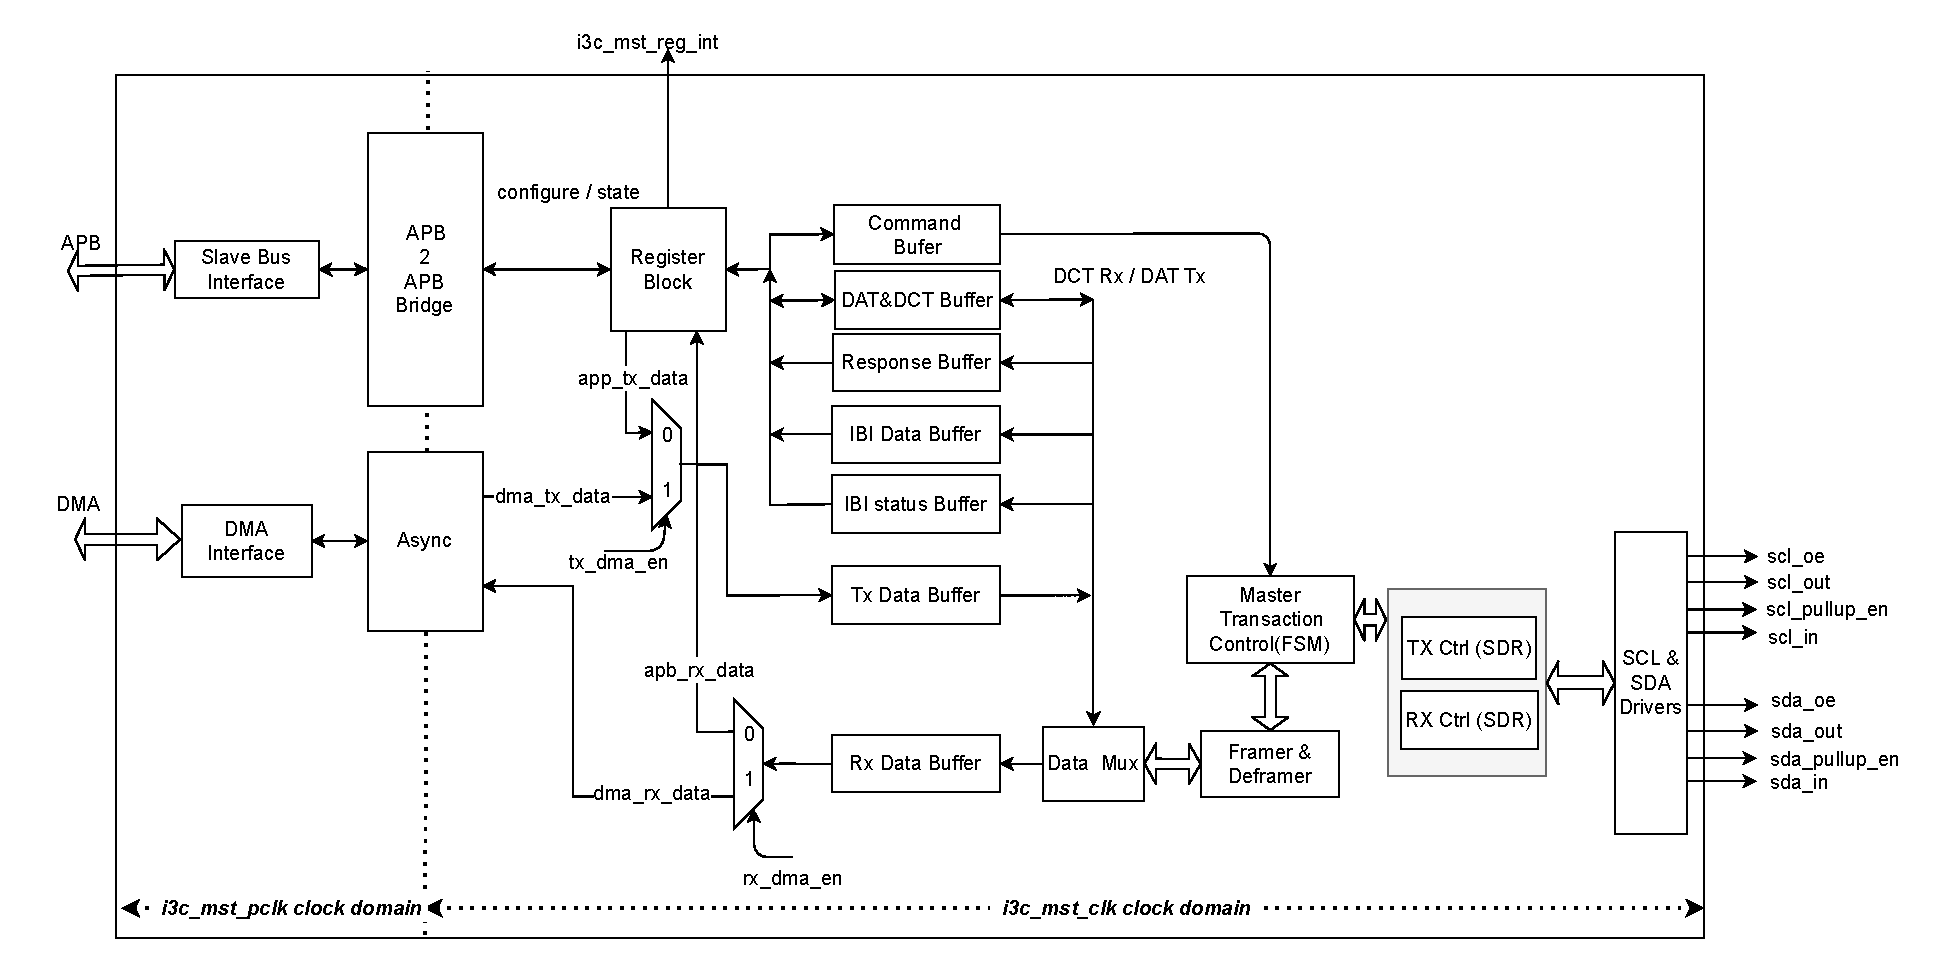
\includegraphics[width=1.0\linewidth]{47-I3C//figures/47-I3C_BlockDiagram__EN}
    \caption{I3C Controller Block Diagram}
    \label{fig:i3c_mst_digram}
\end{figure}



The I3C controller is divided into the APB clock domain (i.e., i3c\_mst\_pclk clock domain) and the core clock domain (i.e., i3c\_mst\_core\_clk clock domain). Figure \ref{fig:i3c_mst_digram} shows the structure in \chipname{} I3C controller, consisting of:

\begin{itemize}
    \item DMA Interface: Asserts and de-asserts the handshake interface of AHB GDMA, based on the occupancy levels of the asynchronous FIFO.
    \item Async Module and APB Bridge: Maintains coherency between the APB clock and core clock.
    \item Register Block: Programs the controller for different modes such as I2C-compatible and I3C-specific modes, and enables or disables interrupts. It serves as the interface for transmitting commands, the Dynamic Address table, and Tx-data, as well as receiving the device characteristic table, Rx-data, and responses from the Controller.
    \item Command Buffer: Stores commands to initiate a specified transfer.
    \item DAT Buffer: Stores Dynamic Addresses for I3C targets and Static Addresses for Legacy I2C devices. These addresses are crucial for identifying and communicating with different devices on the bus.
    \item DCT Buffer: Stores device characteristics returned from I3C targets.
    \item Response Buffer: Stores the response and status of I2C or I3C transfers.
    \item IBI Data Buffer: Stores IBI data from targets with In-Band Interrupts.
    \item IBI Status Buffer: Stores status information when In-Band interrupts occur.
    \item Tx Data Buffer: Stores data to be transmitted.
    \item Rx Data Buffer: Stores received data.
    \item Data Mux: Selects the sources of sent data and the destination of received data.
    \item Framer and Deframer: Packs and splits data from the transaction layer and the buffer controller.
    \item TX Ctrl: Transmits data from the Framer to the bus.
    \item RX Ctrl: Receives data from the SDA line.
    \item Master Transaction Control (FSM):
    \begin{itemize}
      \item Executes commands stored in the command buffer, which are pre-configured instructions for data transfer operations.
      \item Generates a timing sequence that conforms to the I3C protocol, ensuring correct synchronization of data transmission and reception.
      \item Controls the framing of sent data and the deframing of received data, maintaining data integrity during the transfer process.
      \item Controls the TX Ctrl or Rx Ctrl modules to transmit or receive data on the SDA pin, coordinating overall data flow on the bus.
    \end{itemize}
\end{itemize}




%%%%%%%%%%%%%%%%%%%%%%%%%%%%%%
%%% Functional Description %%%
%%%%%%%%%%%%%%%%%%%%%%%%%%%%%%
\section{Functional Description}
\label{sec:i3c-func-descr}

\subsection{Clock Configuration}

The I3C master clock (i3c\_mst\_clk) can be sourced from three different clock inputs, which determine the maximum frequency of the I3C Serial Clock (SCL). The SCL frequency is generated by dividing the selected master clock.

The master clock source is selected via \hyperref[fielddesc:HPSYSCLKRSTI3CMSTCLKSRCSEL]{HP\_SYS\_CLKRST\_I3C\_MST\_CLK\_SRC\_SEL} in the \hyperref[mod:resclk]{Reset and Clock} chapter. The available sources are:

\begin{itemize}
    \item XTAL\_40M\_CLK: Suitable for scenarios requiring low power consumption and moderate data transfer speeds.
    \item REF\_120M\_CLK: Designed for applications needing a relatively fast data transfer rate but not the highest data transfer rate.
    \item REF\_160M\_CLK: Ideal for applications demanding the highest data transfer speeds, providing optimal performance for high-speed applications.
\end{itemize}

Details regarding the frequencies and the selection mechanism are elaborated in the \hyperref[mod:resclk]{Reset and Clock} chapter.

\subsection{Data Structure}
The I3C controller defines the following data structures:
\begin{itemize}
    \item Command Descriptor Data Structure
    \item Response Descriptor Data Structure
    \item IBI Descriptor Data Structure
    \item DAT Data Structure
    \item DCT Data Structure
\end{itemize}

\subsubsection{Command Descriptor Data Structure}

The I3C controller initiates Common Command Code (CCC) transfers, private transfers, and dynamic address assignment via the Command Descriptor, which is written into the Command Buffer through the \hyperref[regdesc:I3CMSTMEMCOMMANDBUFPORTREG]{I3C\_COMMAND\_PORT\_REG}. All Command Descriptors fall into one of the following three categories:


\begin{itemize}
    \item \textbf{Address Assignment}: Used for Dynamic Address assignment.
    \item \textbf{Regular Trans}: Used for CCC transfer and private data transfer.
    \item \textbf{Immediate Data Trans}: Used only for write transfers, not for read transfers. The command contains the data to be transmitted, enabling immediate transfer of small data packets without requiring additional buffer operations.
\end{itemize}

As shown in Figure \ref{fig:cmd_structure}, the I3C controller defines a 64-bit command descriptor structure for each command type. Each descriptor schedules a command transaction to a target device on the I3C bus.

The \textbf{COMMAND\_L} field represents the lower 32 bits of the descriptor and defines the low-word layout for all supported I3C commands; the \textbf{COMMAND\_H} field represents the upper 32 bits and defines the corresponding high-word layout. Each command type is described in one row of the structure table.


\begin{figure}[H]
    \centering
    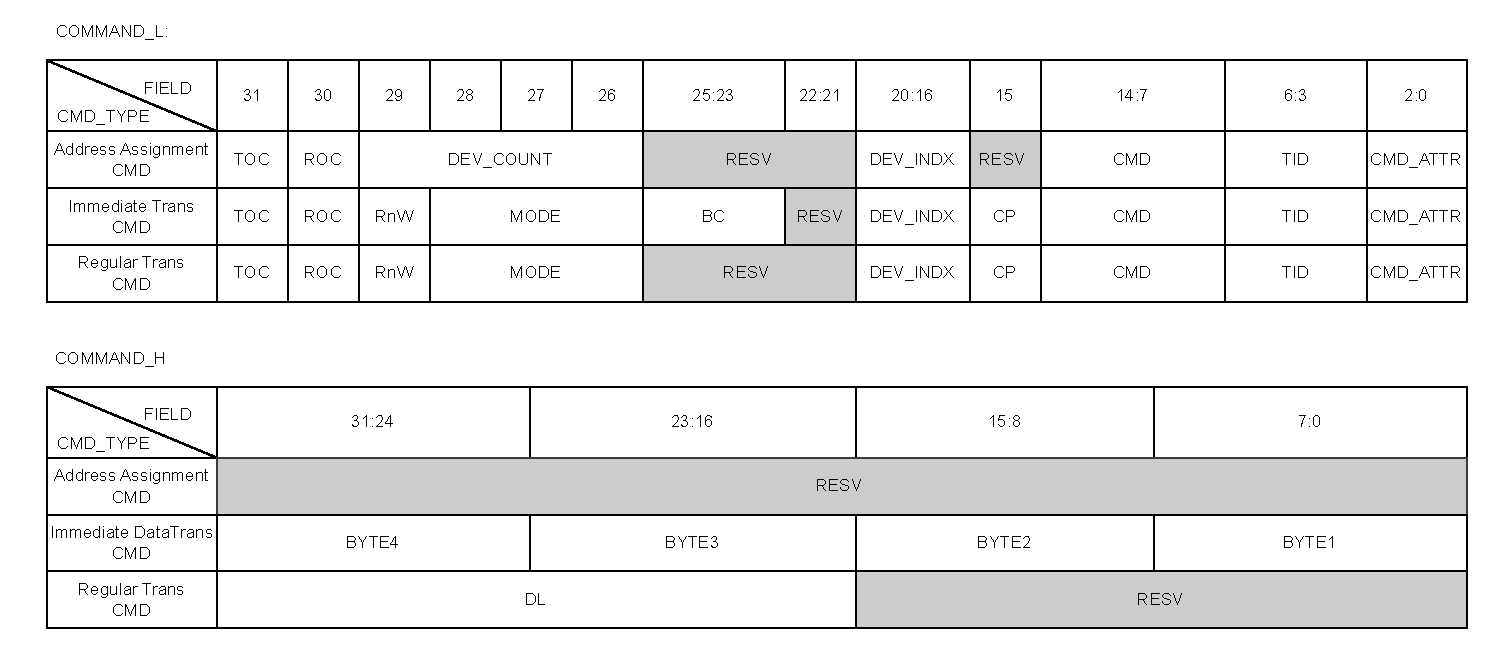
\includegraphics[width=1.0\linewidth]{47-I3C//figures/47-I3C_command_structure__EN}
    \caption{Command Descriptor Data Structure}
    \label{fig:cmd_structure}
\end{figure}

The description of each field in the command descriptor data structure is as follows:
\begin{itemize}
    \item \textbf{CMD\_ATTR:}
    \begin{itemize}
        \item 0: Regular Trans. Commonly used in general CCC transfer and private data transfer scenarios.
        \item 1: Immediate Trans. Suitable for situations where a small amount of data needs to be transferred quickly, with data directly included in the command.
        \item 2: Address Assignment. Specifically used for the dynamic address assignment operation of target devices. When a new device joins the I3C bus, the I3C controller uses this mode to assign a unique address to the device.
    \end{itemize}
    \item \textbf{TID:} Transaction ID. Used as an identification tag for this command. The same value should be reflected in the \textbf{Response Descriptor}.
    \item \textbf{CMD:} Transfer Command CCC Value, specifies CCC code.
    \item \textbf{CP:} Command Present. Indicates whether the \textbf{CMD} field is valid for CCC transfer.
    \begin{itemize}
        \item 0: This structure describes an SDR transfer, so the CMD field is invalid.
        \item 1: This structure describes a CCC transfer, so the CMD field is valid.
    \end{itemize}
    \item \textbf{DEV\_INDEX:} Indicates the DAT table index for the target device being addressed with the transfer. Static and device addressing information will be stored at this index in the DAT. This field is reserved in Broadcast CCC transfer.
    \item \textbf{RESV:} Reserved.
    \item \textbf{DEV\_COUNT:} Indicates the number of devices to which a Dynamic Address shall be assigned.
    \item \textbf{RnW:} Identifies the direction of this transfer.
    \begin{itemize}
        \item 0: Write transfer
        \item 1: Read transfer
    \end{itemize}
    \item \textbf{BC}: Indicates the number of bytes in COMMAND\_H.
    \item \textbf{MODE:} Data Transfer Speed and Mode. Sets the mode and speed for the I3C or I2C transfer. Interpretation of this field depends on whether the device is in I3C Mode or I2C Mode (see the DEVICE field in the DAT Table entry indexed by field DEV\_INDEX).\\
    Values for I3C Mode:
    \begin{itemize}
        \item I3C SDR0: Standard SDR speed, its timing registers are REG\_I3C\_PP\_LOW\_PERIOD and REG\_I3C\_PP\_HIGH\_PERIOD.
        \item I3C SDR1–4: Lower SDR Speed; timing register is REG\_I3C\_EXT\_LOW\_PERIOD1–4.
    \end{itemize}
    Values for I2C Mode:
    \begin{itemize}
        \item 0x0: I2C Fast Mode, its timing registers are REG\_I2C\_FM\_LOW\_PERIOD and REG\_I2C\_FM\_HIGH\_PERIOD.
        \item 0x1: I2C Fast Mode+, its timing registers are REG\_I2C\_FMP\_LOW\_PERIOD and REG\_I2C\_FMP\_HIGH\_PERIOD.
    \end{itemize}
    \item \textbf{ROC:} Response on Completion, controls whether the response status is sent after the successful completion of the transfer command.
    \begin{itemize}
        \item 0: Response Status is not required.
        \item 1: Response Status is required.
    \end{itemize}
    \item \textbf{TOC:} Terminate on Completion, controls what bus condition to issue after the transfer command completes. This field must be set to 1 for ENTDAA.
    \begin{itemize}
        \item 0: Issue Repeated Start (Sr) at the end of transfer.
        \item 1: Issue Stop (P) at the end of transfer.
    \end{itemize}
    \item \textbf{DL:} Data Length, indicates the number of bytes to be transferred.
    \item \textbf{BYTE1-4}: Data Byte1–4 for Immediate Data Transfer.
\end{itemize}


\subsubsection{Response Descriptor Data Structure}

The Response Descriptor, shown in Figure \ref{fig:resp-structure}, is a read-only structure that describes the success or failure of a transfer command and the amount of data transferred. The I3C controller returns the status of the transfer command into the Response Buffer using this data structure. You can read the Response Descriptor via the \hyperref[regdesc:I3CMSTMEMRESPONSEBUFPORTREG]{I3C\_MST\_RESP\_BUFFER\_PORT\_REG}.

\begin{figure}[H]
    \centering
    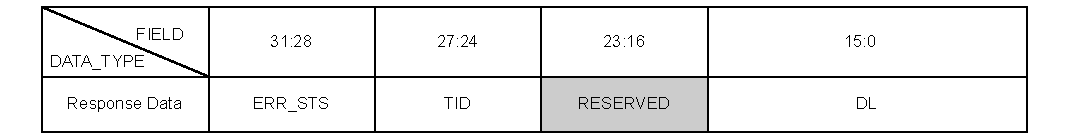
\includegraphics[width=1\linewidth]{47-I3C//figures/47-I3C_RESP_STRUCTURE__EN}
    \caption{Response Descriptor Data Structure}
    \label{fig:resp-structure}
\end{figure}

Each field in the response descriptor structure is described as follows:
\begin{itemize}
    \item \textbf{DL}, Data Length. The meaning of this field depends on the context:
    \begin{itemize}
        \item For Write Transfer: Remaining data length (in bytes)
        \item For Read Transfer: Received data length (in bytes)
        \item For Address Assignment: Remaining Devices count
    \end{itemize}
    \item \textbf{TID}, Identification tag for the command. This value must match one of the commands sent on the bus. Values:
    \begin{itemize}
        \item 0 \verb+~+ 15: Valid Transaction IDs
    \end{itemize}
    \item \textbf{ERR\_STS}, Error Type. It indicates the response status, either success or the error type encountered for the processed command.
    \begin{itemize}
        \item 0: No Error
        \item 1 \verb+~+ 2: Reserved
        \item 3: Read Data Length mismatch
        \item 4: I3C Broadcast Address NACK Error
        \item 5: Address NACK or Dynamic Address Assignment NACK
        \item 6: Rx Data Buffer Overflow/Tx Data Buffer Underflow
        \item 7 \verb+~+ 8: Reserved
        \item 9: I2C Slave Write Data NACK Error
        \item 10 \verb+~+ 15: Reserved
    \end{itemize}
\end{itemize}

\subsubsection{IBI Status Descriptor Data Structure}

The IBI status descriptor, shown in Figure \ref{fig:ibi-data-structure}, is a read-only structure that describes an IBI event received from a target device on the I3C bus. The I3C controller returns the status of the received In-Band Interrupts (IBI) into the IBI Buffer using this data structure. You can read the IBI Descriptor via the \hyperref[regdesc:I3CMSTMEMIBISTATUSBUFREG]{I3C\_MST\_MEM\_IBI\_STATUS\_BUF\_REG}.

\begin{figure}[H]
    \centering
    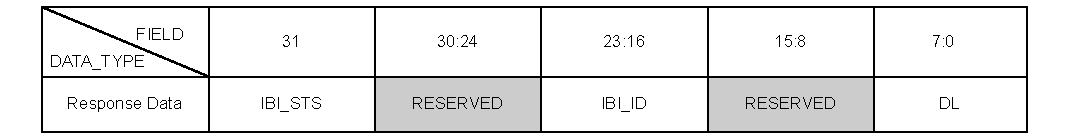
\includegraphics[width=1\linewidth]{47-I3C//figures/47-I3C_IBI_STRUCTURE__EN}
    \caption{IBI Status Descriptor Data Structure}
    \label{fig:ibi-data-structure}
\end{figure}

Each field in the IBI status descriptor data structure is described as follows:

\begin{itemize}
    \item \textbf{DL}, Data Length. Number of data bytes in the received IBI data.
    \item \textbf{IBI\_ID}, IBI Identifier received after START, containing the target's device address and R/W bit.
    \item \textbf{IBI\_STS}, IBI status.
    \begin{itemize}
        \item 0: IBI ACK. The IBI was handled with ACK.
        \item 1: IBI NACK. The IBI was handled with NACK.
    \end{itemize}
\end{itemize}

\subsubsection{DAT Data Structure}

The DAT table stores the Device Address of the devices attached to the I3C Bus, along with several control and information fields per device. The software populates the DAT table with these data structures, as shown in Figure \ref{fig:dat_i3c_dyn_sta} and Figure \ref{fig:dat_i2c_ds}. DAT table entries are indexed by the DEV\_INDEX field in the command descriptor; the controller accesses the corresponding device information through this index during Dynamic Address Assignment and other transfers.

Per-device prioritization of IBIs from targets can be set via the dynamic address value programmed by software.

The following three types of data structures are supported in the Device Address Table:

\begin{itemize}
\item The first type is shown in Figure \ref{fig:dat_i3c_dyn_sta} for I3C devices with a Static Address.
    \begin{itemize}
         \item \textbf{Static Address}: Static Address of the I3C Target.
         \item \textbf{Dynamic Address}:
         \begin{itemize}
             \item If used for address assignment by SETDASA CCC, it is the Dynamic Address to be assigned to the I3C device with a Static Address.
             \item For other transfers, the Dynamic Address is used as the target's address.
         \end{itemize}
         \item \textbf{DNRC}: Device NACK Retry Counter. It determines the number of retries when the current transfer is nacked.
         \item \textbf{Bit[31]}: 0. It indicates the I3C device.
    \end{itemize}

\begin{figure}[H]
    \centering
    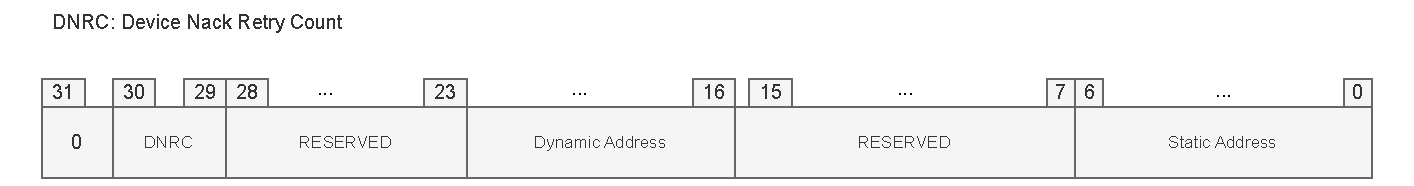
\includegraphics[width=1\linewidth]{47-I3C//figures/47-I3C_DAT_I3C_DYN_STA}
    \caption{DAT Structure for I3C Target with Static Address}
    \label{fig:dat_i3c_dyn_sta}
\end{figure}

\item The second type is shown in Figure \ref{fig:dat_i3c_only_dyn} for Pure I3C devices with a Dynamic Address.
      \begin{itemize}
       \item \textbf{Dynamic Address}:
             \begin{itemize}
                 \item If used for address assignment by ENTDAA CCC, it is the Dynamic Address to be assigned to the I3C device without a Static Address.
                 \item For other transfers, the Dynamic Address is used as the target's address.
             \end{itemize}
       \item \textbf{PAR}: Parity Bit of the 7-bit Dynamic Address.
       \item \textbf{DNRC}: Device NACK Retry Counter. It determines the number of retries when the current transfer is nacked.
       \item \textbf{Bit[31]}: 0. Indicates the I3C device.
     \end{itemize}
\end{itemize}

\begin{figure}[H]
    \centering
    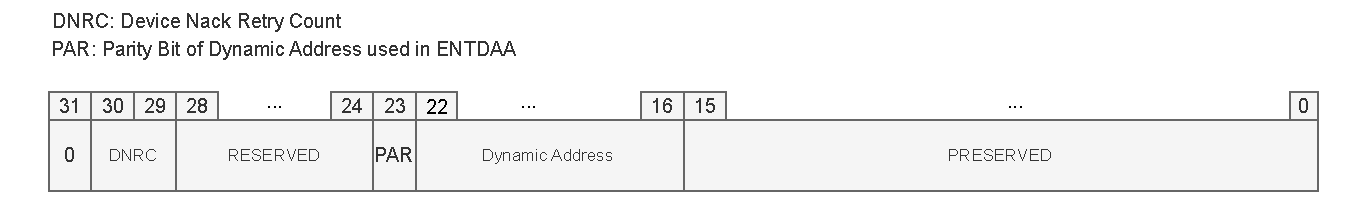
\includegraphics[width=1\linewidth]{47-I3C//figures/47-I3C_DAT_I3C_ONLY_DYN}
    \caption{DAT Data Structure for Pure I3C Target without Static Address}
    \label{fig:dat_i3c_only_dyn}
\end{figure}
\begin{itemize}

\item The third type is shown in Figure \ref{fig:dat_i2c_ds} for I2C devices with a Static Address.
      \begin{itemize}
       \item \textbf{Static Address}: Static Address of the I2C device.
       \item \textbf{DNRC}: Device NACK Retry Counter. It determines the number of retries when the current transfer is nacked.
       \item \textbf{Bit[31]}: 1. Indicates the I2C device.
     \end{itemize}
\end{itemize}
\begin{figure}[H]
    \centering
    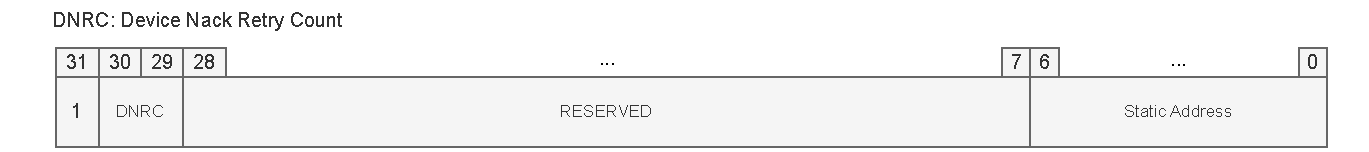
\includegraphics[width=1\linewidth]{47-I3C//figures/47-I3C_DAT_I2C_DS}
    \caption{DAT Data Structure for I2C Slave}
    \label{fig:dat_i2c_ds}
\end{figure}

\subsubsection{DCT Data Structure}

The DCT table captures the Device Characteristics (PID, BCR, DCR) and the assigned Dynamic Address of each device on the I3C bus that participates in the Dynamic Address Allocation (ENTDAA) procedure. The I3C controller receives the bytes transmitted by ENTDAA in the order they appear on the bus. By default, the first received bit is stored in the least significant bit position. In word data storage mode, the Little-Endian convention is followed, meaning the bytes received first are stored in the low-address part (low-index positions) of the word, and the subsequently received bytes are stored in sequence towards the high-address direction to form the complete word data. As shown in Figure \ref{fig:dct_structure}, the DCT allocates four entries for each device.

\begin{figure}[H]
    \centering
    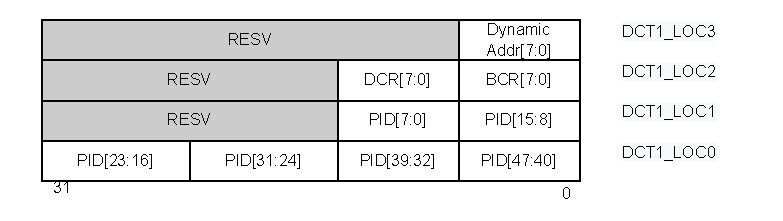
\includegraphics[width=0.8\linewidth]{47-I3C//figures/47-I3C_DCT}
    \caption{DCT Data Structure}
    \label{fig:dct_structure}
\end{figure}

\subsection{Data Conversion}

A data shifter in RX Ctrl and TX Ctrl performs serial/parallel conversion. It converts byte data in the TX Data Buffer to an outgoing serial bit stream or an incoming serial bit stream to byte data in the DCT table, RX Data Buffer, and IBI Data Buffer.
\begin{itemize}
    \item Configure \hyperref[fielddesc:I3CMSTREGRXBITORDER]{I3C\_MST\_REG\_RX\_BIT\_ORDER} to select the storage order of the received bits.
    \item Configure \hyperref[fielddesc:I3CMSTREGRXBYTEORDER]{I3C\_MST\_REG\_RX\_BYTE\_ORDER} to select either little-endian or big-endian format.
\end{itemize}

\subsection{DAT and DCT Memory Control}

The DCT table is write-only for the I3C controller and read-only for the CPU. The DAT Table is write-only for the CPU and read-only for the I3C controller. The DAT table and DCT table share a 60×32-bit RAM, where the first 48 entries (offsets 0–47) are allocated to the DCT table and the last 12 entries (offsets 48–59) are allocated to the DAT table.

As shown in Figure \ref{fig:dct_dat_ram}, each entry in this RAM maps to a unique port register accessible by the CPU:

\begin{itemize}
    \item DAT Table: \hyperref[regdesc:I3CMSTMEMDEVADDRTABLENLOCREG]{I3C\_MST\_MEM\_DEV\_ADDR\_TABLE\regindex{n}\_LOC\_REG} (\regindex{n}: 1–12)
    \item DCT Table: \hyperref[regdesc:I3CMSTMEMDEVCHARTABLENLOCMREG]{I3C\_MST\_MEM\_DEV\_CHAR\_TABLE\regindex{n}\_LOC\regindex{m}\_REG} (\regindex{n}: 1–12, \regindex{m}: 1–4)
\end{itemize}
\begin{figure}[H]
    \centering
    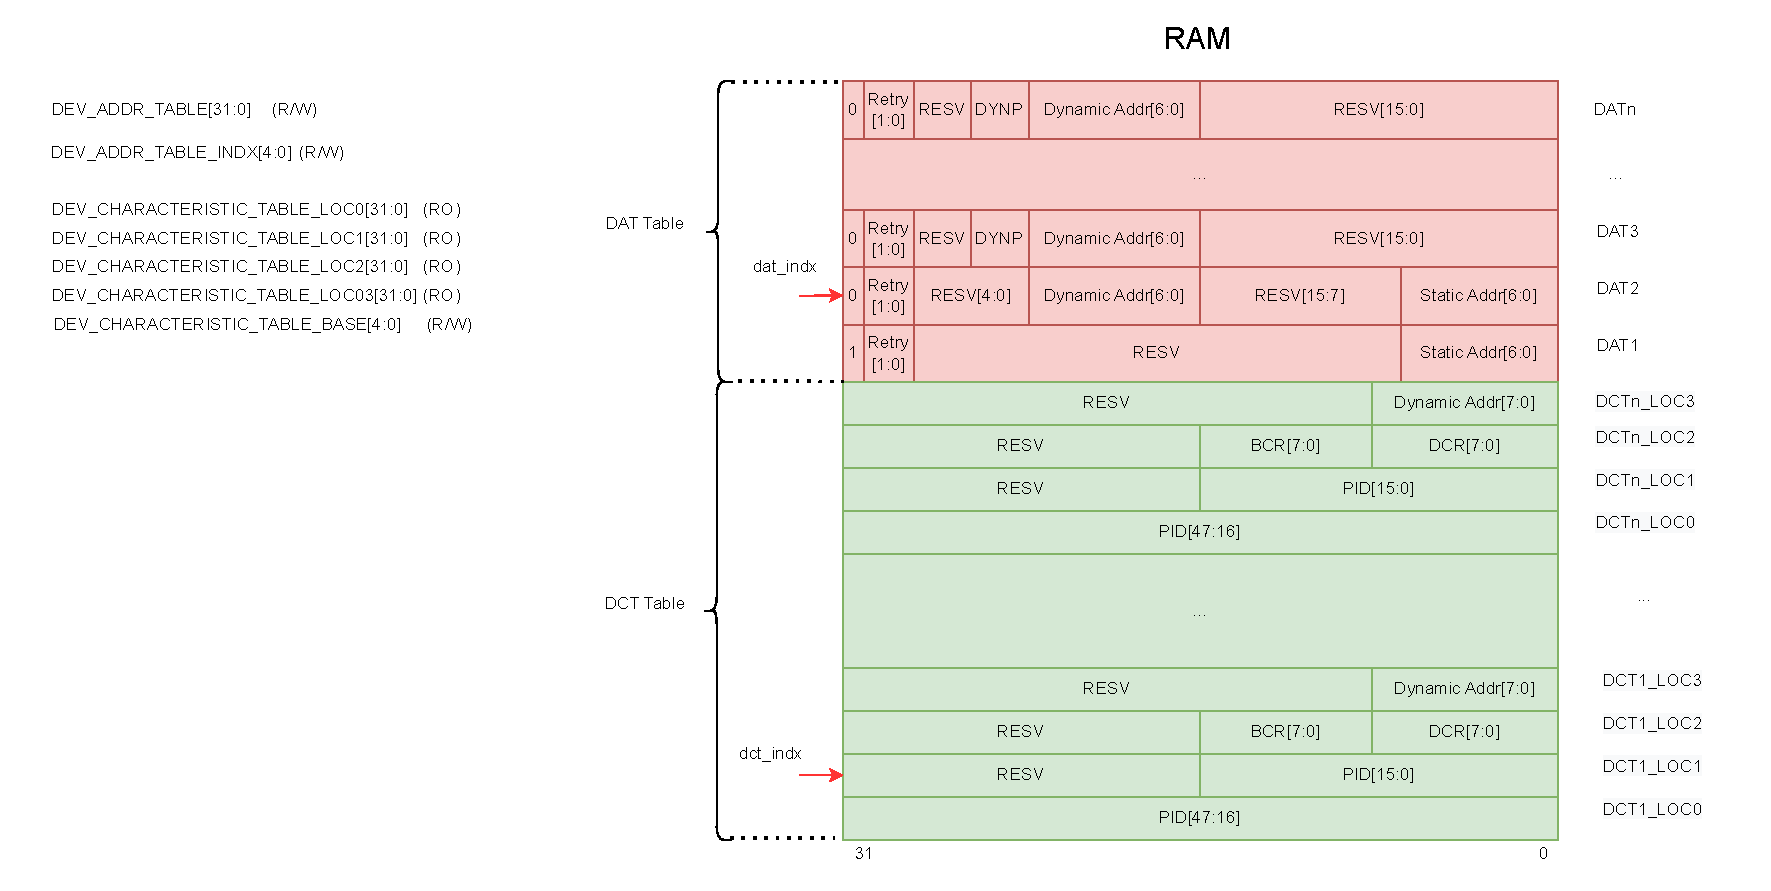
\includegraphics[width=1.0\linewidth]{47-I3C/figures/47-I3C_DAT_DCT_BUF}
    \caption{DAT and DCT Sharing RAM}
    \label{fig:dct_dat_ram}
\end{figure}

During dynamic address assignment using the ENTDAA CCC command, the dat\_indx and dct\_indx values indicate the positions in the DAT and DCT buffers where the I3C controller stores the dynamic address and device characteristics of the target that wins arbitration, respectively. The initial values of dat\_indx and dct\_indx can be configured through the R/W fields \hyperref[fielddesc:I3CMSTREGDATDAAINITINDEX]{I3C\_MST\_REG\_DAT\_DAA\_INIT\_INDEX} and \hyperref[fielddesc:I3CMSTREGDCTDAAINITINDEX]{I3C\_MST\_REG\_DCT\_DAA\_INIT\_INDEX} in \hyperref[regdesc:I3CMSTDEVICETABLEREG]{I3C\_MST\_DEVICE\_TABLE\_REG}, respectively.

After address assignment, the current dat\_indx and dct\_indx values can be read through the RO fields \hyperref[fielddesc:I3CMSTPRESENTDATINDEX]{I3C\_MST\_PRESENT\_DAT\_INDEX} and \hyperref[fielddesc:I3CMSTPRESENTDCTINDEX]{I3C\_MST\_PRESENT\_DCT\_INDEX} in \hyperref[regdesc:I3CMSTDEVICETABLEREG]{I3C\_MST\_DEVICE\_TABLE\_REG}, respectively.

\subsection{TX/RX Data Storage}

Both the TX Data Buffer and RX Data Buffer are 32×32-bit and operate in FIFO mode. The TX Data Buffer is write-only for the CPU or AHB GDMA (enable DMA TX by setting \hyperref[fielddesc:I3CMSTREGDMATXEN]{I3C\_MST\_REG\_DMA\_TX\_EN}) and read-only for the I3C controller. It stores data from the CPU or AHB DMA in transmission order. During a regular write transfer, the I3C controller reads the specified length of data from the TX Data Buffer and transmits it sequentially through the SDA line. The CPU populates the TX Data Buffer via \hyperref[fielddesc:I3CMSTMEMTXDATAPORT]{I3C\_MST\_MEM\_TX\_DATA\_PORT}.

The RX Data Buffer is write-only for the controller and read-only for the CPU or AHB GDMA (enable DMA RX by setting \hyperref[fielddesc:I3CMSTREGDMARXEN]{I3C\_MST\_REG\_DMA\_RX\_EN}). It stores data received from the SDA in a specified order, which is determined by \hyperref[fielddesc:I3CMSTREGRXBITORDER]{I3C\_MST\_RX\_BIT\_ORDER} and \hyperref[fielddesc:I3CMSTREGRXBYTEORDER]{I3C\_MST\_RX\_BYTE\_ORDER}.

Both TX and RX Data Buffers can store up to 128 bytes at a time. For transmissions exceeding 128 bytes, the TX Data Buffer must be refilled in a timely manner based on \hyperref[int:TXDATABUFTHLDINT]{TX\_DATA\_BUF\_THLD\_INT}, and the RX Data Buffer must be read in a timely manner based on \hyperref[int:RXDATABUFTHLDINT]{RX\_DATA\_BUF\_THLD\_INT}. The TX threshold must ensure that the TX Data Buffer is replenished before it becomes empty, while the RX threshold must ensure that data is read before the RX Data Buffer overflows. Otherwise, the transmission will fail.

\subsection{DMA Mode}

When the I3C controller sends and receives bulk data, using Direct Memory Access (DMA) mode improves efficiency. To use DMA correctly, follow these configuration steps and notes:

\begin{enumerate}
    \item Enable DMA channels:
    \begin{itemize}
        \item Configure \texttt{I3C\_MST\_REG\_DMA\_TX\_EN} and \texttt{I3C\_MST\_REG\_DMA\_RX\_EN} to enable the controller's TX and RX DMA channels, respectively;
        \item Note: DMA transfers data only — it does not transfer commands or status information.
    \end{itemize}

    \item Command and AHB GDMA linked-list preparation:
    \begin{itemize}
        \item After enabling the DMA TX and RX modes, the CPU must first cache commands in the command buffer;
        \item Configure the transmit and receive linked lists of the AHB GDMA (Advanced High-performance Bus General-purpose DMA) as required.
        \item Start the transmission. The AHB GDMA and I3C controller will then work together to complete data sending and receiving.
    \end{itemize}

    \item Configure AHB GDMA
    \begin{itemize}
        \item Configure the receive (RX) channel:
        \begin{itemize}
            \item Before RX begins, configure the receive linked list;
            \item Point \texttt{GDMA\_INLINK\_ADDR\_CHn} to the first receive linked-list descriptor and set \texttt{GDMA\_INLINK\_START\_CHn};
            \item After start, the I3C controller transfers received data to the AHB GDMA, and AHB GDMA stores it at the locations specified by the receive linked list.
        \end{itemize}

        \item Configure the transmit (TX) channel:
        \begin{itemize}
            \item Before TX begins, prepare the transmit linked list and the data to be sent;
            \item Point \texttt{GDMA\_OUTLINK\_ADDR\_CHn} to the first transmit linked-list descriptor and set \texttt{GDMA\_OUTLINK\_START\_CHn};
            \item After start, the GDMA engine reads data from the transmit linked list and provides it to the I3C controller, which transmits the data over the SDA line.
        \end{itemize}
    \end{itemize}

    \item Data length and alignment rules:
    \begin{itemize}
        \item The TX/RX data length is determined by the "Data Length" field in the command descriptor;
        \item The I3C controller and AHB GDMA interact in words; transfers are word-aligned;
        \item When "Data Length" is not an integer multiple of a word: in RX the I3C controller pads with 0 to achieve word alignment; in TX the AHB GDMA may pad with invalid data, but the I3C controller will extract and send only the valid bytes specified by "Data Length".
    \end{itemize}
\end{enumerate}

\subsection{Transfer Types}

The I3C controller is an SDR-only peripheral, following bus communication protocols to transfer data between master and target.

\subsubsection{Dynamic Address Assignment (DAA)}

As the main master, the I3C controller performs a Dynamic Address Assignment (DAA) procedure to provide a unique Dynamic Address to each I3C device connected to the I3C Bus. Once a device receives a Dynamic Address, this assigned Dynamic Address is used in all subsequent transactions until the master changes it.

As shown in Figure \ref{fig:daa_trans_format}, there are two DAA methods:
\begin{itemize}
    \item SETDASA
    \item ENTDAA
\end{itemize}
\begin{figure}[H]
    \centering
    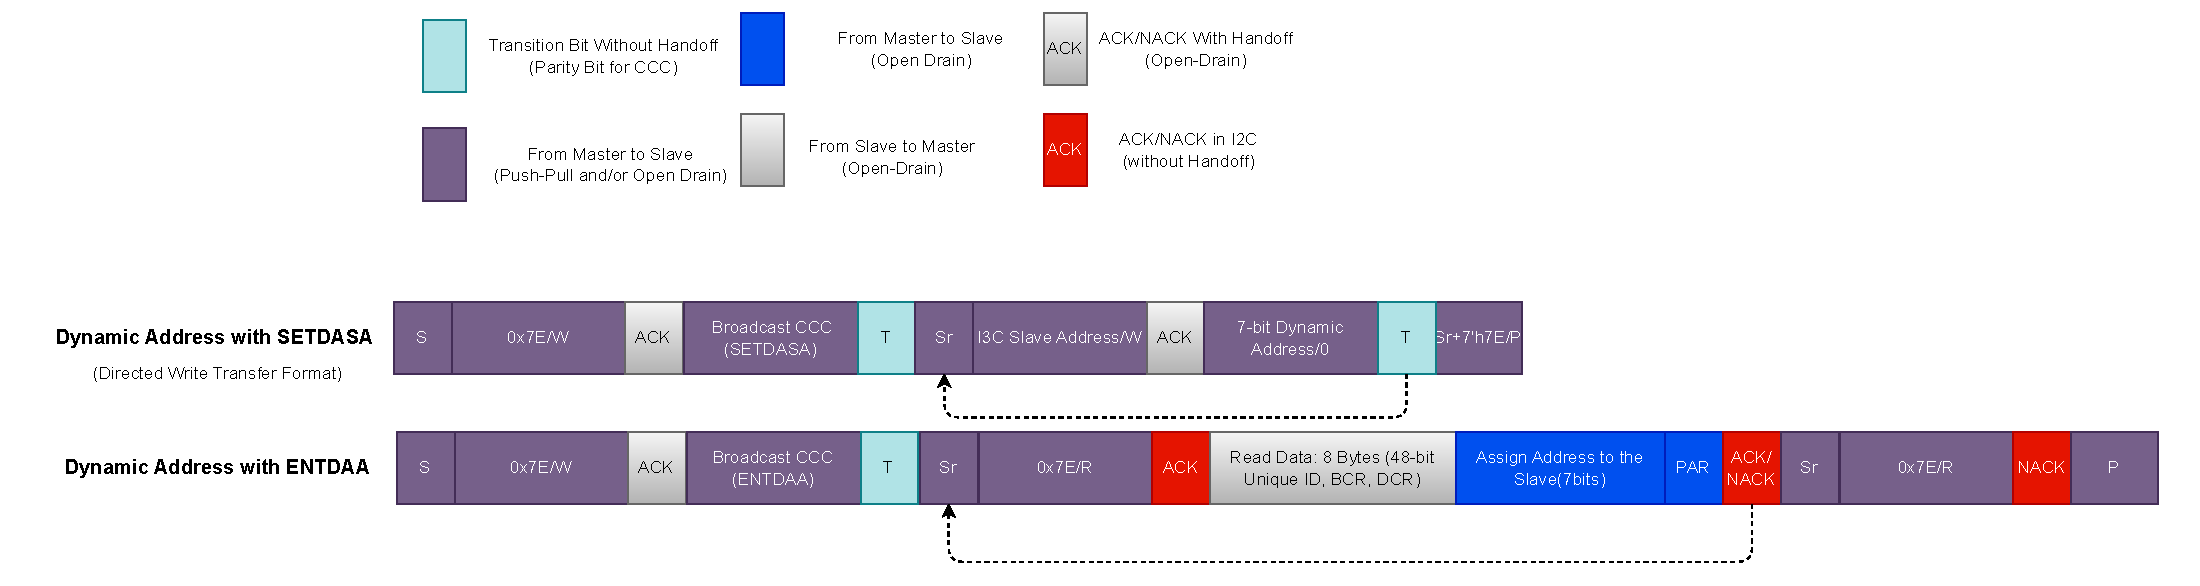
\includegraphics[width=1\linewidth]{47-I3C/figures/47-I3C_DAA}
    \caption{Address Assignment Transfer Format}
    \label{fig:daa_trans_format}
\end{figure}

\subparagraph{SETDASA Procedure}

SETDASA is one of the directed common command codes that allows the main master to assign a Dynamic Address to any I3C device with a known Static Address. This method is faster than using the ENTDAA procedure.

\subparagraph{ENTDAA Procedure}

The main master assigns Dynamic Addresses to I3C devices that do not yet have one by issuing the broadcast ENTDAA Common Command Code (CCC). This procedure is performed after cold power-up and follows the SETDASA process used to assign Dynamic Addresses to Static Address devices.

The main master may issue one or multiple ENTDAA commands to complete Dynamic Address assignment for all connected I3C devices. The number of devices that can be assigned per command is constrained by the sizes of the DAT Table and DCT Table, with an upper limit of 12 devices.

\subsubsection{CCC Transfer}

Common Command Codes (CCCs) are globally supported commands that can be transmitted either directly to a specific I3C target device or to all I3C target devices simultaneously.

The Command Code space is divided into Broadcast Commands and Direct Commands:
\begin{itemize}
    \item Broadcast CCC Commands are Common Codes 0x00 to 0x7F
    \item Direct CCC Commands are Command Codes from 0x80 to 0xFE
\end{itemize}

Both CCC commands always start with the I3C Broadcast Address (7-bit address 0x7E). That is, after START or Repeated START, the Address of a CCC command is always 0x7E, and the RnW bit is always a Write.

\subparagraph{Direct CCC Transfer}

The Direct CCC transfer format is shown in Figure \ref{fig:i3c_trans_format}. A Direct Write CCC is directed to one or more specific I3C Targets, selected by the Target Dynamic Address(es). A Direct Read CCC reads data from one or more specific I3C Targets, selected by the Target Dynamic Address(es). Every Direct CCC command ends with STOP or a Repeated START, followed by the I3C Broadcast Address (0x7E).

\subparagraph{Broadcast CCC Transfer}

The Broadcast CCC transfer format is shown in Figure \ref{fig:i3c_trans_format}. A Broadcast Write CCC is seen by all I3C Targets. Every Broadcast Write CCC command ends with a Repeated START or a STOP, except ENTDAA, which always ends with a STOP.

\begin{figure}[H]
    \centering
    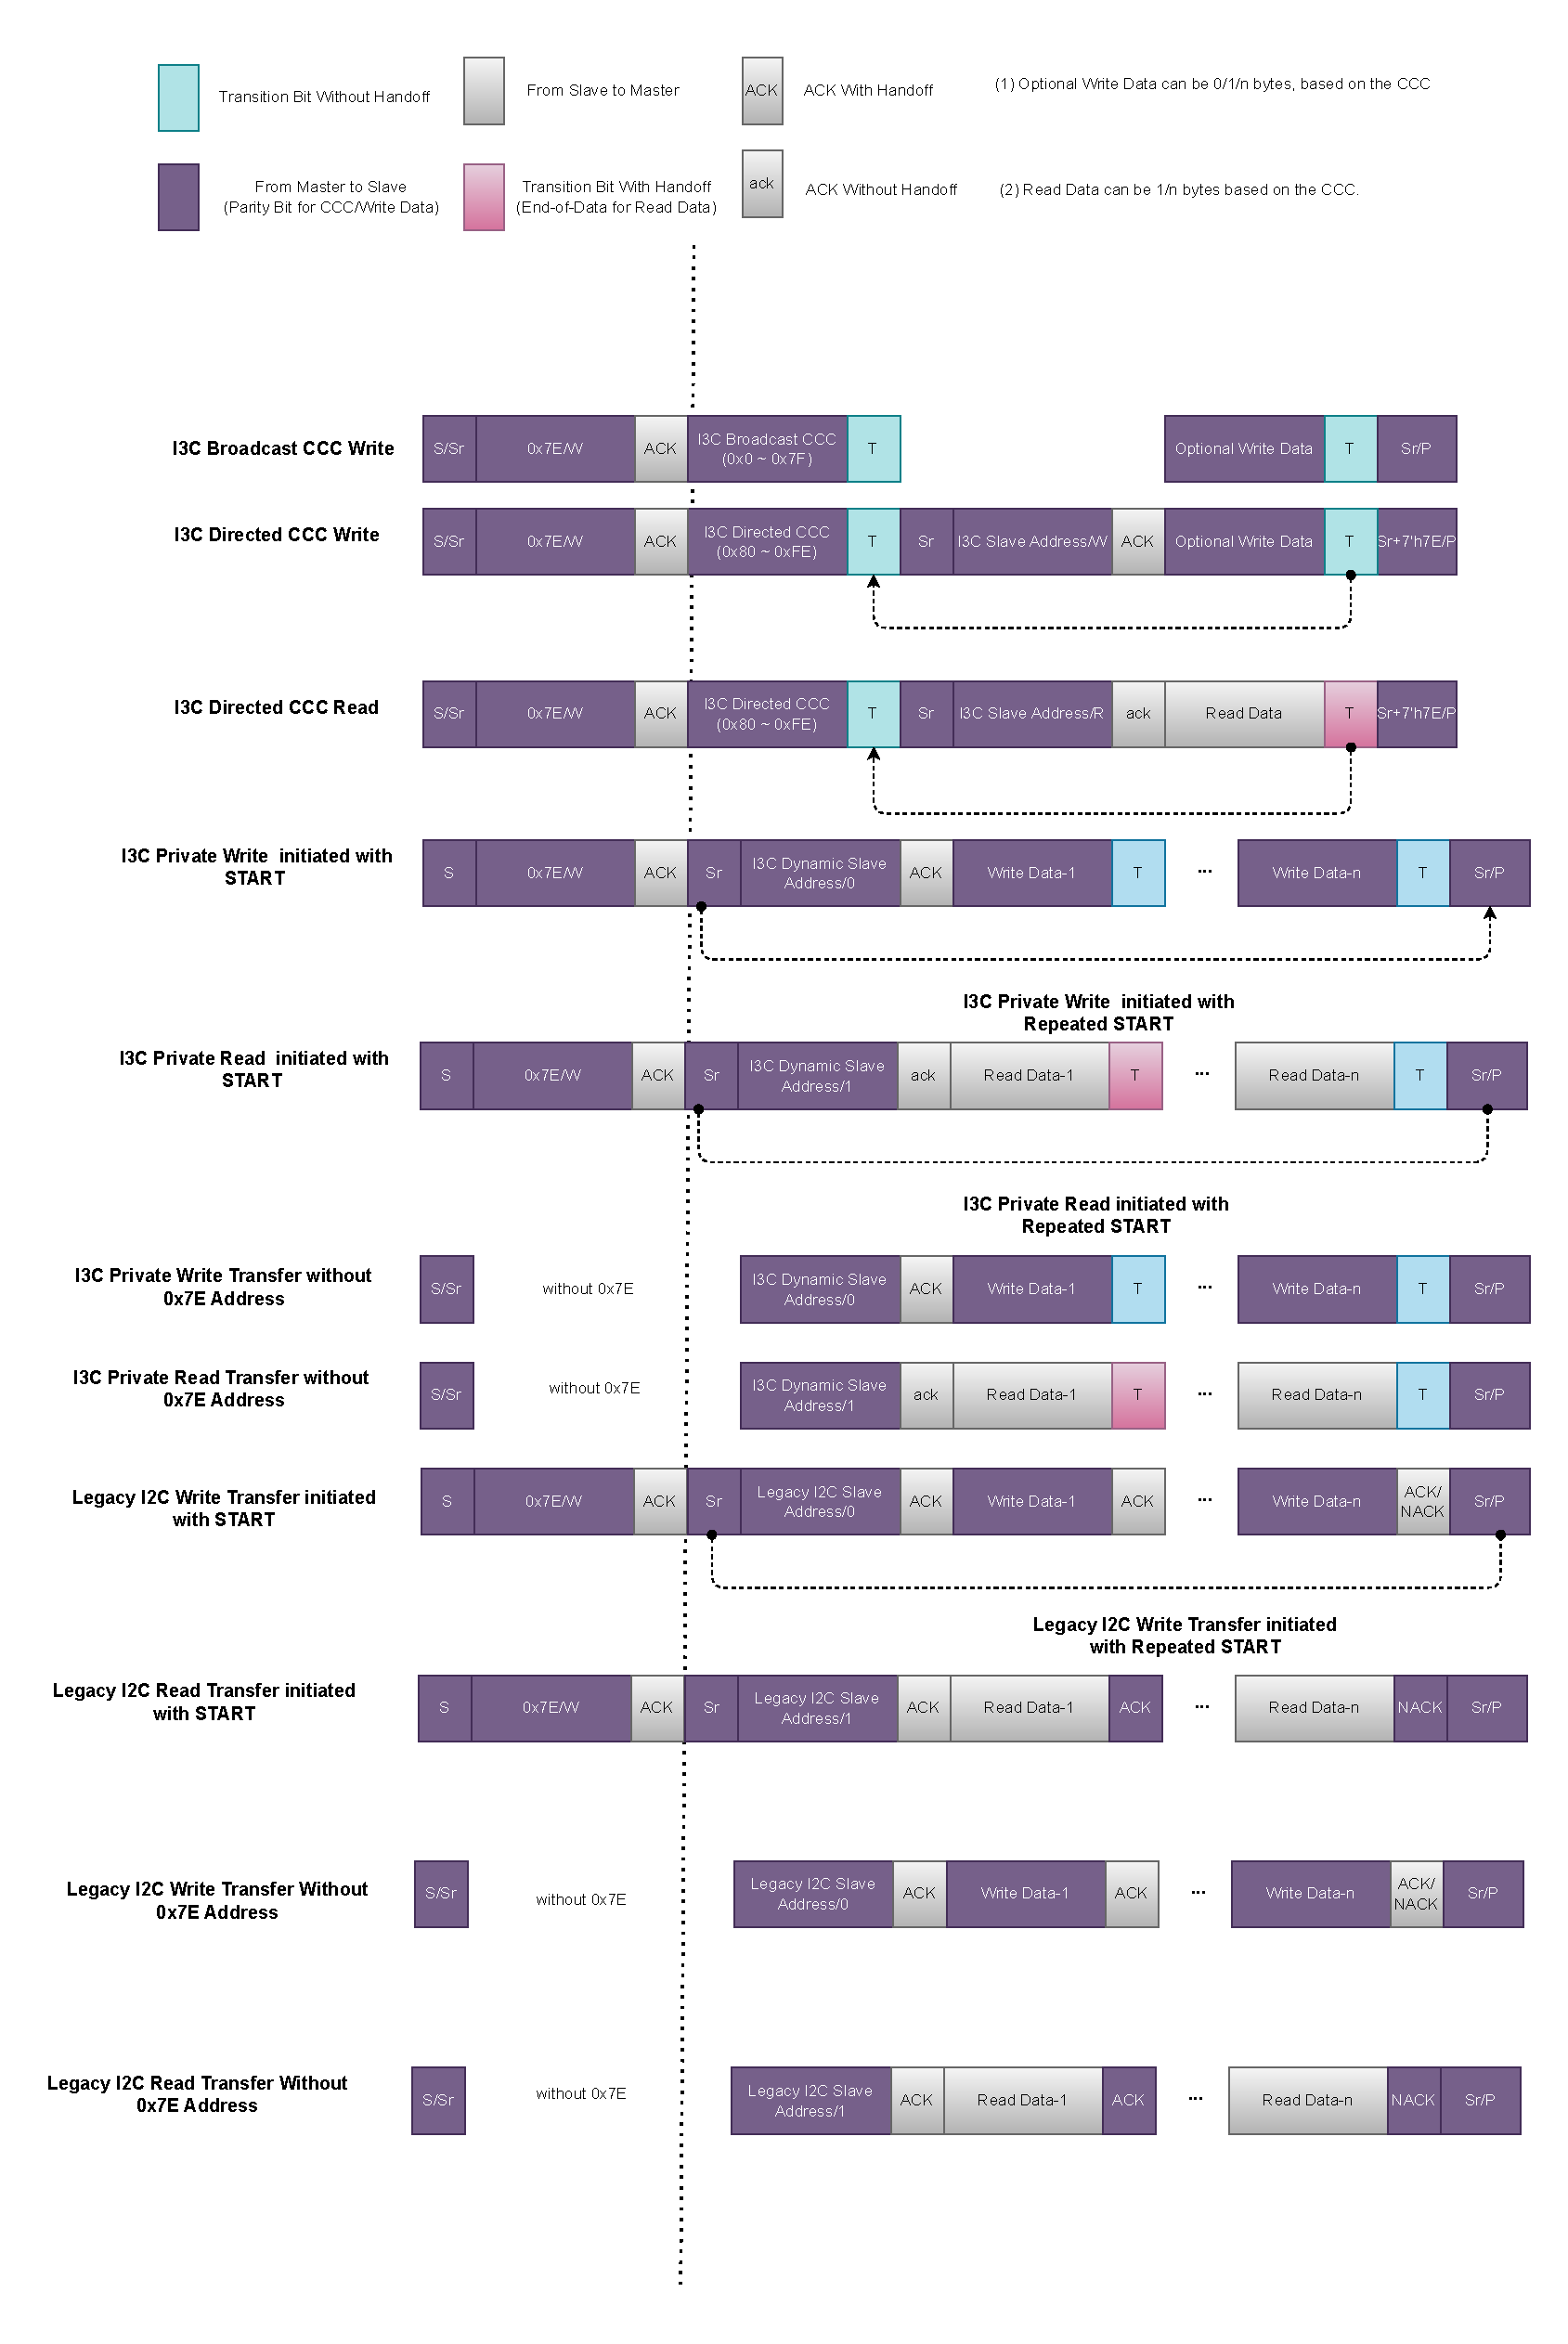
\includegraphics[width=0.8 \linewidth]{47-I3C//figures/47-I3C_Format}
    \caption{I3C Transfer Format}
    \label{fig:i3c_trans_format}
\end{figure}

\subsubsection{Private Data Transfer}

As shown in Figure \ref{fig:i3c_trans_format} , I3C can initiate private transfers like I2C transfers without CCC. If \hyperref[fielddesc:I3CMSTREGBAINCLUDE]{I3C\_MST\_BA\_INCLUDE} is set to 1, the I3C Controller can include a Broadcast Address Head for private transfers. If the broadcast address is not included, then IBIs driven from targets might not win the arbitration, potentially delaying acceptance of the IBIs.

\subsubsection{Legacy I2C Transfer}

The I3C Controller uses the I2C protocol to initiate the I2C transfers for Legacy I2C devices. The I3C Controller can include a Broadcast Address Head for I2C transfers by setting the \hyperref[fielddesc:I3CMSTREGBAINCLUDE]{I3C\_MST\_BA\_INCLUDE} to allow priority for the IBI from I3C devices.

\subsubsection{In-band Interrupt (IBI) Handling}

The I3C Controller supports only Slave Interrupt Request (SIR), which is a unique type (the assigned Dynamic Address with the Read flag set). There are two 32-bit vector control registers in the I3C Controller:

\begin{itemize}
    \item \hyperref[regdesc:I3CMSTIBISIRREQREJECTREG]{I3C\_MST\_SIR\_REQ\_REJECT}: Controls the response individually for each I3C target device.
    \item \hyperref[regdesc:I3CMSTIBISIRREQPAYLOADREG]{I3C\_MST\_SIR\_REQ\_PAYLOAD}: Indicates whether an IBI payload follows an IBI request from the I3C target device.
\end{itemize}

Each bit in the above registers is mapped to a unique Dynamic Address assigned to the I3C target device on the bus through modular arithmetic, as shown in the formula below.

This modular operation limits the Dynamic Address range of the I3C target device, but allows the I3C controller to handle in-band interrupts from various I3C targets flexibly.

\textbf{IBI\_Index = mod32\{IBI\_DYNAMIC\_ADDR[6:5]+IBI\_DYNAMIC\_ADDR[4:0]\}}\\

SIR\_x is a bit in the register, assumed to be mapped to the I3C target device I3C\_SLV\_y after the modular operation.

\subparagraph{ACK SIR}
When SIR\_x in \hyperref[regdesc:I3CMSTIBISIRREQREJECTREG]{I3C\_MST\_SIR\_REQ\_REJECT} is set to 0, the I3C Controller responds to the SIR from I3C\_SLV\_y with ACK and generates an IBI status response in the IBI Status Buffer to notify the application. If SIR\_x in \hyperref[regdesc:I3CMSTIBISIRREQPAYLOADREG]{I3C\_MST\_SIR\_REQ\_PAYLOAD} is set to 1, the I3C controller also receives the mandatory byte following SIR into the IBI Data Buffer.

\subparagraph{NACK SIR}
When SIR\_x in \hyperref[regdesc:I3CMSTIBISIRREQREJECTREG]{I3C\_MST\_SIR\_REQ\_REJECT} is set to 1, the I3C Controller responds to the SIR from I3C\_SLV\_y with NACK. If \hyperref[fielddesc:I3CMSTREGAUTODISIBIEN]{I3C\_MST\_AUTO\_DIS\_IBI\_EN} is set to 1, the I3C Controller can generate a directed DISEC CCC to the SIR-initiated device after the SIR is NACKed.

If \hyperref[fielddesc:I3CMSTREGIBIRSTARTTRANSEN]{I3C\_MST\_IBI\_RSTART\_TRANS\_EN} is set to 1, the I3C controller continues to execute the command that was previously interrupted by the IBI after the IBI is completed.

\subsection{Timing Configuration}
The I3C Controller provides a set of timing configuration registers that allow software to precisely configure the SCL clock waveform, SDA data setup/hold timing, and bus condition (START, STOP, Bus Free) timing based on the I3C master clock (i3c\_mst\_clk).

\subsubsection{Count Unit Convention}
All timing registers are expressed in units of i3c\_mst\_clk clock cycles. The internal counter starts at 1 and triggers a state transition when the count value is $\geq$ the register setting, therefore:
\begin{equation}
    T_\text{actual} = (\text{register value} + 1) \times T_\text{clk}
    \label{eq:timing_unit}
\end{equation}
where $T_\text{clk} = 1/f_\mathrm{i3c\_mst\_clk}$.
\subsubsection{Timing Registers}
I3C Common Timing Register:
\begin{itemize}
    \item \hyperref[fielddesc:I3CMSTREGSCLSTARTHOLDTIME]{I3C\_MST\_SCL\_START\_HOLD\_TIME}: Specifies the interval between the moment SDA is pulled low and the moment SCL is pulled low when the I3C Controller generates a START condition.
    \item \hyperref[fielddesc:I3CMSTREGSCLRSTARTSETUPTIME]{I3C\_MST\_SCL\_RSTART\_SETUP\_TIME}: Specifies the interval between the positive edge of SCL and the negative edge of SDA for a RESTART condition.
    \item \hyperref[fielddesc:I3CMSTREGSCLSTOPHOLDTIME]{I3C\_MST\_SCL\_STOP\_HOLD\_TIME}: Specifies the delay time after the STOP condition.
    \item \hyperref[fielddesc:I3CMSTREGSCLSTOPSETUPTIME]{I3C\_MST\_SCL\_STOP\_SETUP\_TIME}: Specifies the time between the rising edge of SCL and the rising edge of SDA.
\end{itemize}

I3C Open Drain Timing Register:

\begin{itemize}
    \item \hyperref[fielddesc:I3CMSTREGI3CMSTODLOWPERIOD]{I3C\_MST\_OD\_LOW\_PERIOD}: Specifies the SCL Open-Drain low period for I3C Target transfers.
    \item \hyperref[fielddesc:I3CMSTREGI3CMSTODHIGHPERIOD]{I3C\_MST\_OD\_HIGH\_PERIOD}: Specifies the SCL Open-Drain high period for I3C Target transfers.
    \item \hyperref[fielddesc:I3CMSTREGI2CFMLOWPERIOD]{I3C\_MST\_I2C\_FM\_LOW\_PERIOD}: Specifies the SCL Open-Drain low period for legacy I2C Target transfers in I2C Fast Mode.
    \item \hyperref[fielddesc:I3CMSTREGI2CFMHIGHPERIOD]{I3C\_MST\_I2C\_FM\_HIGH\_PERIOD}: Specifies the SCL Open-Drain high period for legacy I2C Target transfers in I2C Fast Mode.
    \item \hyperref[fielddesc:I3CMSTREGI2CFMPLOWPERIOD]{I3C\_MST\_I2C\_FMP\_LOW\_PERIOD}: Specifies the SCL Open-Drain low period for legacy I2C Target transfers in I2C Fast Plus Mode.
    \item \hyperref[fielddesc:I3CMSTREGI2CFMPHIGHPERIOD]{I3C\_MST\_I2C\_FMP\_HIGH\_PERIOD}: Specifies the SCL Open-Drain high period for legacy I2C Target transfers in I2C Fast Plus Mode.
    \item \hyperref[fielddesc:I3CMSTREGSDAODSAMPLETIME]{I3C\_MST\_SDA\_OD\_SAMPLE\_TIME}: Specifies the interval between the rising edge of SCL in Open-Drain mode and the level sampling time of SDA for I3C Target transfers. It is advised to set a value in the middle of SCL's high period, so as to correctly sample the level of SDA.
    \item \hyperref[fielddesc:I3CMSTREGSDAODTXHOLDTIME]{I3C\_MST\_SDA\_OD\_TX\_HOLD\_TIME}: Specifies the interval that SDA output level must be held after the falling edge of SCL in Open-Drain mode.
\end{itemize}

I3C Push-Pull Timing Register:
\begin{itemize}
    \item \hyperref[fielddesc:I3CMSTREGI3CMSTPPHIGHPERIOD]{I3C\_MST\_PP\_HIGH\_PERIOD}: Specifies the SCL Push-Pull high period for I3C Target transfers in all SDR mode.
    \item \hyperref[fielddesc:I3CMSTREGI3CMSTPPLOWPERIOD]{I3C\_MST\_PP\_LOW\_PERIOD}: Specifies the SCL Push-Pull low period for I3C Target transfers in SDR0 mode.
    \item \hyperref[fielddesc:I3CMSTREGI3CMSTEXTLOWPERIOD1]{I3C\_MST\_EXT\_LOW\_PERIOD\_*}: Specifies the SCL Push-Pull low period for lower data rate I3C Target transfers:
    \begin{itemize}
        \item \hyperref[fielddesc:I3CMSTREGI3CMSTEXTLOWPERIOD1]{I3C\_MST\_EXT\_LOW\_PERIOD1}: for SDR1 mode.
        \item \hyperref[fielddesc:I3CMSTREGI3CMSTEXTLOWPERIOD2]{I3C\_MST\_EXT\_LOW\_PERIOD2}: for SDR2 mode.
        \item \hyperref[fielddesc:I3CMSTREGI3CMSTEXTLOWPERIOD3]{I3C\_MST\_EXT\_LOW\_PERIOD3}: for SDR3 mode.
        \item \hyperref[fielddesc:I3CMSTREGI3CMSTEXTLOWPERIOD4]{I3C\_MST\_EXT\_LOW\_PERIOD4}: for SDR4 mode.
    \end{itemize}
    \item \hyperref[fielddesc:I3CMSTREGI3CMSTTERMNTEXTLOWTIME]{I3C\_MST\_TERMN\_T\_EXT\_LOW\_TIME}: Add the required extended SCL Push-Pull low period value based on \hyperref[fielddesc:I3CMSTREGI3CMSTPPLOWPERIOD]{I3C\_MST\_I3C\_MST\_PP\_LOW\_PERIOD} for the I3C read termination bit.
\end{itemize}




%%%%%%%%%%%%%%%%%%%%%
%%% Interrupts %%%
%%%%%%%%%%%%%%%%%%%%%

\section{Interrupts}


\chipname{}'s I3C Controller can generate the following interrupt signal(s) that will be sent to the \href{mod:intmtrx}{Interrupt Matrix}.

    \begin{itemize}
        \item I3C\_MST\_INTR
    \end{itemize}

Several internal interrupt sources from the I3C Controller can generate the above interrupt signal. Table \ref{tab:i3c_controller-int-sources} lists the interrupt sources, their trigger conditions, and the resulting interrupt signal(s).

\begin{longtable}{ | L{4.5cm} | L{8.5cm} | L{2.5cm} | }
\caption{I3C Controller's Internal Interrupt Sources} \label{tab:i3c_controller-int-sources}
\\ \hline
\rowcolor{lightgray}
\textbf{Internal Interrupt Source} & \textbf{Trigger Condition}  &  \textbf{Interrupt Signal}\\ \hline
\label{int:CMDCCCMISMATCHINT}CMD\_CCC\_MISMATCH\_INT  &  The CCC in the command does not match the command type. The CMD field of the Address Assignment Command can only be filled with ENTDAA and SETDASA. &  I3C\_MST\_INTR  \\ \hline
\label{int:IBIDETECTINT}IBI\_DETECT\_INT &  IBI request detected & I3C\_MST\_INTR \\ \hline
\label{int:IBIHANDLEDONEINT}IBI\_HANDLE\_DONE\_INT &  IBI request processing completed  & I3C\_MST\_INTR \\ \hline
\label{int:IBISTATUSBUFOVFINT}IBI\_STATUS\_BUF\_OVF\_INT &  IBI Status overflowed & I3C\_MST\_INTR \\ \hline
\label{int:IBIDATABUFOVFINT}IBI\_DATA\_BUF\_OVF\_INT &  IBI Data Buffer overflowed  & I3C\_MST\_INTR \\ \hline
\label{int:RESPBUFOVFINT}RESP\_BUF\_OVF\_INT &  Response Buffer overflowed & I3C\_MST\_INTR \\ \hline
\label{int:DETECTSTARTINT}DETECT\_START\_INT &  The START flag is detected on the bus  & I3C\_MST\_INTR \\ \hline
\label{int:COMMANDDONEINT}COMMAND\_DONE\_INT &  Just one command executed  & I3C\_MST\_INTR \\ \hline
\label{int:TRANSFERCOMPLETEINT}TRANSFER\_COMPLETE\_INT &  A transfer is completed. Depending on the configuration of the TOC bit, a transfer may execute multiple commands in the command buffer.  & I3C\_MST\_INTR \\ \hline
\label{int:TRANSFERERRINT}TRANSFER\_ERR\_INT &  Any error occurs during transfer  & I3C\_MST\_INTR \\ \hline
\label{int:NXTCMDREQERRINT}NXT\_CMD\_REQ\_ERR\_INT &  The controller restarts the next command, but the command buffer is empty. & I3C\_MST\_INTR \\ \hline
\label{int:RESPREADYINT}RESP\_READY\_INT & \begin{itemize}
    \item The number of entries in the Response Buffer is greater than or equal to RESP\_BUF\_THLD.
    \item Or the remaining data in the Response Buffer has not been read for RESP\_BUF\_TO\_VALUE i3c\_mst\_clk's cycles.
\end{itemize}   & I3C\_MST\_INTR \\ \hline
\label{int:CMDBUFEMPTYTHLDINT}CMD\_BUF\_EMPTY\_THLD\_INT &  The number of empty locations in the Command Buffer is greater than or equal to CMD\_EMPTY\_BUF\_THLD  & I3C\_MST\_INTR \\ \hline
\label{int:IBISTATUSTHLDINT}IBI\_STATUS\_THLD\_INT & \begin{itemize}
    \item The number of entries in the IBI Status Buffer is greater than or equal to IBI\_Status\_BUF\_THLD.
    \item Or the number of entries in the IBI Data Buffer is greater than or equal to IBI\_DATA\_BUF\_THLD.
    \item Or the remaining data in the IBI STATUS Buffer has not been read for IBI\_STATUS\_BUF\_TO\_Value i3c\_mst\_clk's cycles.
    \item Or the remaining data in the IBI DATA Buffer has not been read for IBI\_DATA\_BUF\_TO\_Value i3c\_mst\_clk's cycles.
\end{itemize}
   & I3C\_MST\_INTR \\ \hline
\label{int:RXDATABUFTHLDINT}RX\_DATA\_BUF\_THLD\_INT &  \begin{itemize}
    \item The number of entries in the RX Data Buffer is greater than or equal to RX\_BUF\_THLD.
    \item Or the remaining data in the RX Data Buffer has not been read for RX\_DATA\_BUF\_TO\_VALUE i3c\_mst\_clk's cycles.
\end{itemize}   & I3C\_MST\_INTR \\ \hline
\label{int:TXDATABUFTHLDINT}TX\_DATA\_BUF\_THLD\_INT & The number of entries in the TX Data Buffer is less than or equal to TX\_BUF\_THLD. & I3C\_MST\_INTR \\ \hline

\end{longtable}
\begin{tiplisting}
For definitions of \textit{interrupt}, \textit{interrupt signal}, \textit{interrupt source}, and their relationships, refer to Chapter \ref{mod:intmtrx} \textit{\nameref{mod:intmtrx}} > Section \ref{sec:intmtx-int-terminology} \textit{\nameref{sec:intmtx-int-terminology}}.
\end{tiplisting}

%%%%%%%%%%%%%%%%%%%%%%%%%%%%%%
%%% Programming Procedures %%%
%%%%%%%%%%%%%%%%%%%%%%%%%%%%%%

\section{Programming Procedures}
\label{sec:i3c-prog-procedures}
\subsection{Initialize the I3C Controller}

\begin{itemize}
    \item Program the Device Control Register:
    \begin{itemize}
        \item Set \hyperref[fielddesc:I3CMSTREGBAINCLUDE]{I3C\_MST\_BA\_INCLUDE} to 1 to include Address Head (0x7E) in Private Data Transfer as required.
        \item Set \hyperref[fielddesc:I3CMSTREGAUTODISIBIEN]{I3C\_MST\_AUTO\_DIS\_IBI\_EN} to 1 to disable SIR as required.
        \item Set \hyperref[fielddesc:I3CMSTREGDMARXEN]{I3C\_MST\_DMA\_RX\_EN} to 1 to enable DMA RX transfer as required.
        \item Set \hyperref[fielddesc:I3CMSTREGDMATXEN]{I3C\_MST\_DMA\_TX\_EN} to 1 to enable DMA TX transfer as required.
        \item Set \hyperref[fielddesc:I3CMSTREGRXBITORDER]{I3C\_MST\_RX\_BIT\_ORDER} to select the bit order.
        \item Set \hyperref[fielddesc:I3CMSTREGRXBYTEORDER]{I3C\_MST\_RX\_BYTE\_ORDER} to select the byte order.
    \end{itemize}
    \item Program the Timing Control Register. The following timing control registers are based on the i3c\_mst\_clk period:
        \begin{itemize}
          \item I3C Common Timing Register:
          \begin{itemize}
              \item Set the \hyperref[fielddesc:I3CMSTREGSCLSTARTHOLDTIME]{I3C\_MST\_SCL\_START\_HOLD\_TIME} as required.
              \item Set the \hyperref[fielddesc:I3CMSTREGSCLRSTARTSETUPTIME]{I3C\_MST\_SCL\_RSTART\_SETUP\_TIME} as required.
              \item Set the \hyperref[fielddesc:I3CMSTREGSCLSTOPHOLDTIME]{I3C\_MST\_SCL\_STOP\_HOLD\_TIME} as required.
              \item Set the \hyperref[fielddesc:I3CMSTREGSCLSTOPSETUPTIME]{I3C\_MST\_SCL\_STOP\_SETUP\_TIME} as required.
              \item Set the \hyperref[fielddesc:I3CMSTREGSTARTDETHOLDTIME]{I3C\_MST\_START\_DET\_HOLD\_TIME} as required.
              \item Set the \hyperref[fielddesc:I3CMSTREGBUSFREETIME]{I3C\_MST\_BUS\_FREE\_TIME} with the required value for the bus free period.
          \end{itemize}
          \item I3C Open Drain Timing Register:
          \begin{itemize}
              \item Set the \hyperref[fielddesc:I3CMSTREGI3CMSTODLOWPERIOD]{I3C\_MST\_I3C\_MST\_OD\_LOW\_PERIOD} with the required SCL Low Period value for the I3C Open Drain phase.
              \item Set the \hyperref[fielddesc:I3CMSTREGI3CMSTODHIGHPERIOD]{I3C\_MST\_I3C\_MST\_OD\_HIGH\_PERIOD} with the required SCL High Period value for the I3C Open Drain phase.
              \item Set the \hyperref[fielddesc:I3CMSTREGI2CFMLOWPERIOD]{I3C\_MST\_I2C\_FM\_LOW\_PERIOD} with the required SCL Low Period value for I2C Fast Mode.
              \item Set the \hyperref[fielddesc:I3CMSTREGI2CFMHIGHPERIOD]{I3C\_MST\_I2C\_FM\_HIGH\_PERIOD} with the required SCL High Period value for I2C Fast Mode.
              \item Set the \hyperref[fielddesc:I3CMSTREGI2CFMPLOWPERIOD]{I3C\_MST\_I2C\_FMP\_LOW\_PERIOD} with the required SCL Low Period value for I2C Fast Mode Plus.
              \item Set the \hyperref[fielddesc:I3CMSTREGI2CFMPHIGHPERIOD]{I3C\_MST\_I2C\_FMP\_HIGH\_PERIOD} with the required SCL High Period value for I2C Fast Mode Plus.
              \item Set the \hyperref[fielddesc:I3CMSTREGSDAODSAMPLETIME]{I3C\_MST\_SDA\_OD\_SAMPLE\_TIME} with the required SDA sample point for the Open Drain phase.
              \item Set the \hyperref[fielddesc:I3CMSTREGSDAODTXHOLDTIME]{I3C\_MST\_SDA\_OD\_TX\_HOLD\_TIME} with the required SDA Hold Delay for the Open Drain phase.
          \end{itemize}

          \item I3C Push-Pull Timing Register:
          \begin{itemize}
             \item Set the \hyperref[fielddesc:I3CMSTREGI3CMSTPPHIGHPERIOD]{I3C\_MST\_I3C\_MST\_PP\_HIGH\_PERIOD} with the required SCL High Period value for the I3C Push-Pull phase.
             \item Set the \hyperref[fielddesc:I3CMSTREGI3CMSTPPLOWPERIOD]{I3C\_MST\_I3C\_MST\_PP\_LOW\_PERIOD} with the required SCL Low Period value for the I3C Push-Pull phase.
             \item Set \hyperref[fielddesc:I3CMSTREGI3CMSTEXTLOWPERIOD1]{I3C\_MST\_I3C\_MST\_EXT\_LOW\_PERIOD1}, \hyperref[fielddesc:I3CMSTREGI3CMSTEXTLOWPERIOD2]{I3C\_MST\_I3C\_MST\_EXT\_LOW\_PERIOD2}, \hyperref[fielddesc:I3CMSTREGI3CMSTEXTLOWPERIOD3]{I3C\_MST\_I3C\_MST\_EXT\_LOW\_PERIOD3}, and \hyperref[fielddesc:I3CMSTREGI3CMSTEXTLOWPERIOD4]{I3C\_MST\_I3C\_MST\_EXT\_LOW\_PERIOD4} with the required SCL Push-Pull Low Period values for I3C data transfer in SDR1, SDR2, SDR3, and SDR4 speed modes, respectively.
             \item Set \hyperref[fielddesc:I3CMSTREGI3CMSTTERMNTEXTLOWTIME]{I3C\_MST\_I3C\_MST\_TERMN\_T\_EXT\_LOW\_TIME} with the required extended SCL Push-Pull Period value for the I3C read termination bit.
             \item Set the \hyperref[fielddesc:I3CMSTREGSDAPPSAMPLETIME]{I3C\_MST\_SDA\_PP\_SAMPLE\_TIME} with the required SDA sample point for the Push-Pull phase.
             \item Set the \hyperref[fielddesc:I3CMSTREGSDAPPTXHOLDTIME]{I3C\_MST\_SDA\_PP\_TX\_HOLD\_TIME} with the required SDA Hold Delay for the Push-Pull phase.
         \end{itemize}
        \end{itemize}
    \item Programming Buffer Threshold Control Registers:
    \begin{itemize}
        \item Set the \hyperref[fielddesc:I3CMSTREGIBISTATUSBUFTHLD]{I3C\_MST\_IBI\_STATUS\_BUF\_THLD} to the required value.
        \item Set the \hyperref[fielddesc:I3CMSTREGIBIDATABUFTHLD]{I3C\_MST\_IBI\_DATA\_BUF\_THLD} to the required value.
        \item Set the \hyperref[fielddesc:I3CMSTREGRESPBUFTHLD]{I3C\_MST\_RESP\_BUF\_THLD} to the required value.
        \item Set the \hyperref[fielddesc:I3CMSTREGCMDBUFEMPTYTHLD]{I3C\_MST\_CMD\_BUF\_EMPTY\_THLD} to the required value.
        \item Set the \hyperref[fielddesc:I3CMSTREGTXDATABUFTHLD]{I3C\_MST\_TX\_DATA\_BUF\_THLD} to the required value.
        \item Set the \hyperref[fielddesc:I3CMSTREGRXDATABUFTHLD]{I3C\_MST\_RX\_DATA\_BUF\_THLD} to the required value.
    \end{itemize}

    \item Programming Interrupt Registers:
    \begin{itemize}
        \item Enable the related interrupt as required.
    \end{itemize}
    \item Programming Device Address Table:
    \begin{itemize}
        \item The CPU populates the dynamic address to be assigned and the static address of all target devices on the I3C bus according to the DAT Data Structure.
    \end{itemize}
\end{itemize}


\subsection{Dynamic Address Assignment (DAA)}

No data needs to be sent or received during Dynamic Address Assignment. The controller uses Direct SETDASA CCC to assign Dynamic Addresses to I3C Targets with Static Addresses and then uses Broadcast ENTDAA CCC to assign Dynamic Addresses to the remaining I3C Targets.

The controller issues a CCC command according to the command descriptor and reads the dynamic and Static Addresses one by one from the position specified by DEV\_INDEX in the DAT table to DEV\_INDEX + DEV\_COUNT. When executing any DAA command, ensure that the continuous DAT data structure type in the DAT table is the same.

The following are the processes of allocating Dynamic Addresses using SETDASA and ENTDAA respectively.

\subparagraph{SETDASA Transfer}

\begin{itemize}
    \item Programming command descriptor
    \begin{itemize}
        \item Set \textbf{CMD\_ATTR} to 2.
        \item Set \textbf{TID} as required: 0–15.
        \item Set \textbf{CMD} to SETDASA CCC code.
        \item Set \textbf{DEV\_INDEX} to point to the index in the DAT table through which the I3C controller assigns the Dynamic Address to the I3C target with the Static Address.
        \item Set \textbf{DEV\_COUNT} to the maximum number of devices to be addressed with a single command.
        \item Set \textbf{ROC} as required. (0: No response status, 1: Return response status)
        \item Set \textbf{TOC} as required. (0: Issue Repeated Start (Sr), restart next command in Command Buffer; 1: Issue Stop (P), stop the transfer)
        \item Set Reserved field to 0.
    \end{itemize}
    \item Set and then clear \hyperref[fielddesc:I3CMSTREGTRANSSTART]{I3C\_MST\_TRANS\_START} to start the SETDASA CCC transfer.
    \item A \hyperref[int:COMMANDDONEINT]{COMMAND\_DONE\_INT} interrupt is generated when the current command is completed. A \hyperref[int:TRANSFERCOMPLETEINT]{TRANSFER\_COMPLETE\_INT} interrupt is generated when the transfer is completed.
    \item Read Response Status Buffer to check response status.
    \begin{itemize}
        \item After the command is completed, if the ROC bit is set to 1, the transfer status corresponding to COMMAND is stored in the Response Status Buffer.
        \item If a command error occurs, regardless of whether the ROC bit is 1, the transmission status corresponding to the COMMAND is stored in the Response Status Buffer, and a \hyperref[int:TRANSFERERRINT]{TRANSFER\_ERR\_INT} interrupt is generated.
    \end{itemize}
\end{itemize}

\subparagraph{ENTDAA Transfer}
\begin{itemize}
    \item Programming command descriptor
    \begin{itemize}
        \item Set \textbf{CMD\_ATTR} to 2.
        \item Set \textbf{TID} as required: 0–15.
        \item Set \textbf{CMD} to ENTDAA CCC code.
        \item Set \textbf{DEV\_INDEX} to point to the index in the DAT table from which the I3C controller assigns the Dynamic Address to the I3C target that wins the bus arbitration.
        \item Set \textbf{DEV\_COUNT} to the maximum number of devices to be addressed with a single command.
        \item Set \textbf{ROC} as required. (0: No response status, 1: Return response status)
        \item Set \textbf{TOC} to 1.
        \item Set Reserved field to 0.
    \end{itemize}
    \item Set and then clear \hyperref[fielddesc:I3CMSTREGTRANSSTART]{I3C\_MST\_TRANS\_START} to start the ENTDAA CCC transfer.
    \item An interrupt \hyperref[int:COMMANDDONEINT]{COMMAND\_DONE\_INT} is generated when the current command is completed. An interrupt \hyperref[int:TRANSFERCOMPLETEINT]{TRANSFER\_COMPLETE\_INT} is generated when the transfer is completed.
    \item Read Response Status Buffer to check response status.
    \begin{itemize}
        \item After the command is completed, if the ROC bit is set to 1, the transfer status corresponding to COMMAND is stored in the Response Status Buffer.
        \item If a command error occurs, regardless of whether the ROC bit is 1, the transmission status corresponding to the COMMAND is stored in the Response Status Buffer, and a \hyperref[int:TRANSFERERRINT]{TRANSFER\_ERR\_INT} interrupt is generated.
    \end{itemize}
\end{itemize}


\subsection{Direct CCC Transfer}

\subsubsection{Immediate Transfer}
For Direct CCC write transfers without data or with up to 4 bytes of data, use Immediate Transfer.

\begin{itemize}
    \item Programming command descriptor:
    \begin{itemize}
        \item Set \textbf{CMD\_ATTR} to 1.
        \item Set \textbf{TID} as required: 0–15.
        \item Set \textbf{CMD} to the Direct CCC code as required.
        \item Set \textbf{CP} to 1.
        \item Set \textbf{DEV\_INDEX} to point to the respective I3C target address in the DAT table.
        \item Set \textbf{MODE} to the required speed.
        \item Set \textbf{BC} to the number of bytes to be transmitted.
        \item Set \textbf{RnW} to 0.
        \item Set \textbf{ROC} as required.
        \item Set \textbf{TOC} as required.
        \item Set the reserved field to 0.
        \item Fill the data to be sent into \textbf{BYTE1}–\textbf{BYTE4} in order from low to high bytes (fill invalid data with 0).
    \end{itemize}
    \item Set and then clear \hyperref[fielddesc:I3CMSTREGTRANSSTART]{I3C\_MST\_TRANS\_START} to start the Immediate transfer.
    \item A \hyperref[int:COMMANDDONEINT]{COMMAND\_DONE\_INT} interrupt is generated when the current command is completed. A \hyperref[int:TRANSFERCOMPLETEINT]{TRANSFER\_COMPLETE\_INT} interrupt is generated when the transfer is completed.
    \item Read the Response Status Buffer to check the response status:
    \begin{itemize}
        \item After the command is completed, if the ROC bit is set to 1, the transfer status corresponding to the COMMAND will be stored in the Response Status Buffer.
        \item If a command error occurs, regardless of whether the ROC bit is 1, the transmission status corresponding to the COMMAND is stored in the Response Status Buffer, and a \hyperref[int:TRANSFERERRINT]{TRANSFER\_ERR\_INT} interrupt will be generated.
    \end{itemize}
\end{itemize}

\subsubsection{Regular Transfer}
Regular Transfer applies to Direct CCC read and write transfers. If a Direct CCC write transfer needs to send data, fill the data into the TX Data Buffer before the transfer starts.

\begin{itemize}
    \item Programming command descriptor:
    \begin{itemize}
        \item Set \textbf{CMD\_ATTR} to 0.
        \item Set \textbf{TID} as required: 0–15.
        \item Set \textbf{CMD} to the Direct CCC code as required.
        \item Set \textbf{CP} to 1.
        \item Set \textbf{DEV\_INDEX} to point to the respective I3C target address in the DAT table.
        \item Set \textbf{MODE} to the required speed.
        \item Set \textbf{RnW} as required (0: Write, 1: Read).
        \item Set \textbf{ROC} as required.
        \item Set \textbf{TOC} as required.
        \item Set \textbf{DL} to the number of bytes to be sent or received.
        \item Set the reserved field to 0.
        \item For CCC write transfers with data, fill the data (in Word) to be sent into the TX Data Buffer in the order of transmission.
    \end{itemize}
    \item Set and then clear \hyperref[fielddesc:I3CMSTREGTRANSSTART]{I3C\_MST\_TRANS\_START} to start the Direct CCC write or read transfer.
    \item After the transfer starts, for CCC write transfers, the CPU monitors the \hyperref[int:TXDATABUFTHLDINT]{TX\_DATA\_BUF\_THLD\_INT} interrupt and continues to push data to the TX Data Buffer.
    \item For CCC read transfers with data, the CPU monitors the \hyperref[int:RXDATABUFTHLDINT]{RX\_DATA\_BUF\_THLD\_INT} interrupt and then pops the data from the RX Data Buffer.
    \item A \hyperref[int:COMMANDDONEINT]{COMMAND\_DONE\_INT} interrupt is generated when the current command is completed. A \hyperref[int:TRANSFERCOMPLETEINT]{TRANSFER\_COMPLETE\_INT} interrupt is generated when the transfer is completed.
    \item Read the Response Status Buffer to check the response status:
    \begin{itemize}
        \item After the command is completed, if the ROC bit is set to 1, the transfer status corresponding to the COMMAND will be stored in the Response Status Buffer.
        \item If a command error occurs, regardless of whether the ROC bit is 1, the transmission status corresponding to the COMMAND is stored in the Response Status Buffer, and a \hyperref[int:TRANSFERERRINT]{TRANSFER\_ERR\_INT} interrupt will be generated.
    \end{itemize}
\end{itemize}

\subsection{Broadcast CCC Transfer}

\subsubsection{Immediate Transfer}
For a Broadcast CCC write transfer without data or with up to 4 bytes of data, use Immediate Transfer.

\begin{itemize}
    \item Programming command descriptor:
    \begin{itemize}
        \item Set \textbf{CMD\_ATTR} to 1.
        \item Set \textbf{TID} as required: 0–15.
        \item Set \textbf{CMD} to the Broadcast CCC code as required.
        \item Set \textbf{CP} to 1.
        \item Set \textbf{MODE} to the required speed.
        \item Set \textbf{BC} to the number of bytes to be transmitted.
        \item Set \textbf{RnW} to 0.
        \item Set \textbf{ROC} as required.
        \item Set \textbf{TOC} as required.
        \item Set the reserved field to 0.
        \item Fill the data to be sent into \textbf{BYTE1}–\textbf{BYTE4} in order from low to high bytes (fill invalid data with 0).
    \end{itemize}
    \item Set and then clear \hyperref[fielddesc:I3CMSTREGTRANSSTART]{I3C\_MST\_TRANS\_START} to start the Immediate transfer.
    \item A \hyperref[int:COMMANDDONEINT]{COMMAND\_DONE\_INT} interrupt is generated when the current command is completed. A \hyperref[int:TRANSFERCOMPLETEINT]{TRANSFER\_COMPLETE\_INT} interrupt is generated when the transfer is completed.
    \item Read the Response Status Buffer to check the response status:
    \begin{itemize}
        \item After the command is completed, if the ROC bit is set to 1, the transfer status corresponding to the COMMAND will be stored in the Response Status Buffer.
        \item If a command error occurs, regardless of whether the ROC bit is 1, the transmission status corresponding to the COMMAND is stored in the Response Status Buffer, and a \hyperref[int:TRANSFERERRINT]{TRANSFER\_ERR\_INT} interrupt will be generated.
    \end{itemize}
\end{itemize}

\subsubsection{Regular Transfer}
Regular Transfer applies to Broadcast CCC read and write transfers. A Broadcast CCC read transfer only sends commands and does not read data. If a Broadcast CCC write transfer needs to send data, fill the data into the TX Data Buffer before the transfer starts.

\begin{itemize}
    \item Programming command descriptor:
    \begin{itemize}
        \item Set \textbf{CMD\_ATTR} to 0.
        \item Set \textbf{TID} as required: 0–15.
        \item Set \textbf{CMD} to the Broadcast CCC code as required.
        \item Set \textbf{CP} to 1.
        \item Set \textbf{MODE} to the required speed.
        \item Set \textbf{RnW} as required (0: Write, 1: Read).
        \item Set \textbf{ROC} as required.
        \item Set \textbf{TOC} as required.
        \item Set \textbf{DL} to the number of bytes to be sent or received.
        \item Set the reserved field to 0.
        \item For CCC write transfer with data, fill the data (in Word) to be sent into the TX Data Buffer in order of transmission.
    \end{itemize}
    \item Set and then clear \hyperref[fielddesc:I3CMSTREGTRANSSTART]{I3C\_MST\_TRANS\_START} to start the Broadcast CCC write or read transfer.
    \item After the transfer starts, for CCC write transfer, the CPU monitors the \hyperref[int:TXDATABUFTHLDINT]{TX\_DATA\_BUF\_THLD\_INT} interrupt and then continues to push data to the TX Data Buffer.
    \item A \hyperref[int:COMMANDDONEINT]{COMMAND\_DONE\_INT} interrupt is generated when the current command is completed. A \hyperref[int:TRANSFERCOMPLETEINT]{TRANSFER\_COMPLETE\_INT} interrupt is generated when the transfer is completed.
    \item Read the Response Status Buffer to check the response status:
    \begin{itemize}
        \item After the command is completed, if the ROC bit is set to 1, the transfer status corresponding to the COMMAND will be stored in the Response Status Buffer.
        \item If a command error occurs, regardless of whether the ROC bit is 1, the transmission status corresponding to the COMMAND is stored in the Response Status Buffer, and a \hyperref[int:TRANSFERERRINT]{TRANSFER\_ERR\_INT} interrupt will be generated.
    \end{itemize}
\end{itemize}

\subsection{Private Data Transfer}

\subsubsection{Immediate Transfer}
For a private transfer with up to 4 bytes of data, recommend using Immediate Transfer.

\begin{itemize}
    \item Programming command descriptor:
    \begin{itemize}
        \item Set \textbf{CMD\_ATTR} to 1.
        \item Set \textbf{TID} as required: 0–15.
        \item \textbf{CMD} field is reserved.
        \item Set \textbf{CP} to 0.
        \item Set \textbf{DEV\_INDEX} to point to the respective I3C target address in the DAT table.
        \item Set \textbf{MODE} to the required speed.
        \item Set \textbf{BC} to the number of bytes to be transmitted.
        \item Set \textbf{RnW} to 0.
        \item Set \textbf{ROC} as required.
        \item Set \textbf{TOC} as required.
        \item Set the reserved field to 0.
        \item Fill the data to be sent into \textbf{BYTE1}–\textbf{BYTE4} from low to high bytes (fill invalid data with 0).
    \end{itemize}
    \item Set and then clear \hyperref[fielddesc:I3CMSTREGTRANSSTART]{I3C\_MST\_TRANS\_START} to start the Immediate transfer.
    \item A \hyperref[int:COMMANDDONEINT]{COMMAND\_DONE\_INT} interrupt is generated when the current command is completed. A \hyperref[int:TRANSFERCOMPLETEINT]{TRANSFER\_COMPLETE\_INT} interrupt is generated when the transfer is completed.
    \item Read the Response Status Buffer to check the response status:
    \begin{itemize}
        \item After the command is completed, if the ROC bit is set to 1, the transfer status corresponding to the COMMAND will be stored in the Response Status Buffer.
        \item If a command error occurs, regardless of whether the ROC bit is 1, the transmission status corresponding to the COMMAND is stored in the Response Status Buffer, and a \hyperref[int:TRANSFERERRINT]{TRANSFER\_ERR\_INT} interrupt will be generated.
    \end{itemize}
\end{itemize}

\subsubsection{Regular Transfer}
Regular Transfer is applicable to private read and write transfers. For a private write transfer, fill the data to be sent into the TX Data Buffer before the transfer starts.

\begin{itemize}
    \item Programming command descriptor:
    \begin{itemize}
        \item Set \textbf{CMD\_ATTR} to 0.
        \item Set \textbf{TID} as required: 0–15.
        \item \textbf{CMD} field is reserved.
        \item Set \textbf{CP} to 0.
        \item Set \textbf{DEV\_INDEX} to point to the respective I3C target address in the DAT table.
        \item Set \textbf{MODE} to the required speed.
        \item Set \textbf{RnW} as required (0: Write, 1: Read).
        \item Set \textbf{ROC} as required.
        \item Set \textbf{TOC} as required.
        \item Set \textbf{DL} to the number of bytes to be sent or received.
        \item Set the reserved field to 0.
        \item For a private write transfer, fill the data (in Word) to be sent into the TX Data Buffer in the order of transmission.
    \end{itemize}
    \item Set and then clear \hyperref[fielddesc:I3CMSTREGTRANSSTART]{I3C\_MST\_TRANS\_START} to start the write or read transfer.
    \item After the transfer starts, for a private write transfer, the CPU monitors the \hyperref[int:TXDATABUFTHLDINT]{TX\_DATA\_BUF\_THLD\_INT} interrupt and continues to push data to the TX Data Buffer.
    \item For a private read transfer with data, the CPU monitors the \hyperref[int:RXDATABUFTHLDINT]{RX\_DATA\_BUF\_THLD\_INT} interrupt and pops the data from the RX Data Buffer.
    \item A \hyperref[int:COMMANDDONEINT]{COMMAND\_DONE\_INT} interrupt is generated when the current command is completed. A \hyperref[int:TRANSFERCOMPLETEINT]{TRANSFER\_COMPLETE\_INT} interrupt is generated when the transfer is completed.
    \item Read the Response Status Buffer to check the response status:
    \begin{itemize}
        \item After the command is completed, if the ROC bit is set to 1, the transfer status corresponding to the COMMAND will be stored in the Response Status Buffer.
        \item If a command error occurs, regardless of whether the ROC bit is 1, the transmission status corresponding to the COMMAND is stored in the Response Status Buffer, and a \hyperref[int:TRANSFERERRINT]{TRANSFER\_ERR\_INT} interrupt will be generated.
    \end{itemize}
\end{itemize}

\subsection{Legacy I2C Transfer}
Legacy I2C transfer is part of the Private Data Transfer, so the programming procedure is the same. When initializing the DAT table, set DEV\_ADDR\_TABLELOC[31] for I2C transfer to 1 to indicate that the current address is the I2C slave address. Set the DEV\_INDEX to point to the respective I2C slave address in the DAT table.

%%%%%%%%%%%%%%%%%%%%%
%%% Memory Blocks %%%
%%%%%%%%%%%%%%%%%%%%%

\section{Memory Blocks}


The addresses in this section are relative to the I3C controller base address provided in Table \ref{tab:sysmem-base-address} in Chapter \ref{mod:sysmem} \textit{\nameref{mod:sysmem}}.

\begin{longtable}{ | p{3cm} | p{3cm} | r | c | c | c | }
\caption{I3C Master Controller Memory Blocks} \label{dat-dct}
\\ \hline
\rowcolor{lightgray}
Name & Description  &  Size (bytes)  &  Starting Address  &  Ending Address  & Access   \\ \hline
DAT\_MEM\label{TBD1} & Device Address Table  &  48 &  0x00C0  &  0x00EC  &  WR  \\ \hline
DCT\_MEM\label{TBD2} & Device Characteristics Table  &   192  &  0x0100  &  0x01BC  &  RO  \\  \hline
\end{longtable}


%%%%%%%%%%%%%%%%%%%%%%%%
%%% Register Summary %%%
%%%%%%%%%%%%%%%%%%%%%%%%

\newpage
\hypertarget{i3c-reg-summ}{}
\section{Register Summary}
\label{sec:i3c-reg-summ}


The addresses in this section are relative to the I3C controller base address provided in Table \ref{tab:sysmem-base-address} in Chapter \ref{mod:sysmem} \textit{\nameref{mod:sysmem}}.

The abbreviations given in Column \textbf{Access} are explained in Section \hyperref[glossary-access-types]{\textit{Access Types for Registers}}.

\subfile{\modulefiles/47-I3C-mst-reg-summ__EN}
\subfile{\modulefiles/47-I3C-mst-mem-reg-summ__EN}

%%%%%%%%%%%%%%%%%
%%% Registers %%%
%%%%%%%%%%%%%%%%%

\newpage
\section{Registers}

The addresses in this section are relative to the I3C controller base address provided in Table \ref{tab:sysmem-base-address} in Chapter \ref{mod:sysmem} \textit{\nameref{mod:sysmem}}.

For how to program reserved fields, please refer to Section \hyperref[programming-reserved-field]{Programming Reserved Register Field}.


\subfile{\modulefiles/47-I3C-mst-reg__EN}
\subfile{\modulefiles/47-I3C-mst-mem-reg__EN}
\end{document}
